\documentclass[a4paper, 12pt]{article} %tipo de documento e opções gerais
\usepackage[utf8]{inputenc} %codificação
\usepackage[T1]{fontenc} %codificação
\usepackage[portuguese]{babel}  %idioma
\usepackage{amsmath,amssymb,amsfonts,amsthm} %padrões em formato matemático
\usepackage[a4paper,top=3cm,bottom=2cm,left=3cm, right=2cm]{geometry} %margens
\usepackage{indentfirst} %primeiro parágrafo com margem
\usepackage{float} %fixar imagens e tabelas
\usepackage{multicol} %várias colunas
\usepackage{multirow} %várias linhas
\usepackage{graphicx} %colocar imagens 
\usepackage{anyfontsize} %qualquer tamanho de letra
\usepackage{setspace} %espaçamento
\usepackage[titles]{tocloft} %padrões de sumário
\usepackage{fontspec} %outros tipos de fonte
\usepackage{fancyhdr} %padronizar o formato do Header
\usepackage[resetlabels,labeled]{multibib} %bibliografia
\usepackage{newfloat} %alterar nome do quadro
\usepackage{tabls} %pacote para espaçamento de linhas
%\usepackage{titlesec}
\usepackage{makecell}
\usepackage{shadowtext}
\usepackage{eso-pic,graphicx}
\usepackage{tikz} %trabalhar com imagens e add background
\usepackage[absolute,overlay]{textpos}
\usepackage{calc} %para funçoes como \widthof
\usepackage{hyperref}
\usepackage{afterpage} % contracapa
\usepackage{paralist}
\usepackage{enumitem}

\newcommand\blankpage{% código para a contracapa
    \null
    \thispagestyle{empty}%
    \addtocounter{page}{-1}%
    \newpage}

%definindo novo estilo de pagina
\makeatletter
\def\ps@Padrao{
    %número da página com cor clara e no canto
    \def\@oddfoot{\textcolor{white}{\null\hfill\thepage}}%
    \def\@evenfoot{\thepage}%
    %definindo cabeçado para o canto
    \def\@evenhead{\null\hfil\slshape\leftmark }%
    \def\@oddhead{{\slshape\rightmark\hfill 
\includegraphics[scale=0.2]{estat.png}}}} %cabeçalho
\makeatother

\pagestyle{Padrao}

\setmainfont{Arial} %fonte arial
\setstretch{1.5} %espaçamento
\setlength\tablinesep{5pt} %espaço entre as células da tabela

% ALTERANDO O TÍTULO DAS TABELAS E FIGURAS
\addto\captionsenglish{%
  \renewcommand\tablename{Tabela}
  \renewcommand\figurename{Figura}
}
\DeclareFloatingEnvironment[listname=loq, listname={Lista de Quadros}]{quadro}

% ALTERANDO O SUMÁRIO
\makeatletter
\renewcommand\tableofcontents{
  \null\hfill\textbf{\Large\contentsname}\hfill\null\par
  \@mkboth{\MakeUppercase\contentsname}{\MakeUppercase\contentsname}%
  \@starttoc{toc}}
\makeatother	
\addto\captionsenglish{
  \renewcommand{\contentsname}{Sumário}
  }

\clearpage

\begin{document}
\begin{titlepage}

\center
\tikz[remember picture,overlay] \node[opacity=1,inner sep=0pt] at (current page.center){
\includegraphics[width=\paperwidth,height=\paperheight]{capa.png}};

\begin{minipage}{16cm}
\begin{flushright}
% posições do título (substituir o segundo parâmetro do begin{textblock}
% 1 linha:  (4cm, 8.38cm)   nao esquecer de cuidar
% 2 linhas: (4cm, 7.75cm)   do tamanho das fontes
% 3 linhas: (4cm, 7.15cm)   e o espaçamento delas
% 4 linhas: (4cm, 6.55cm)
% 5+ linhas: diminuir tamanho da fonte pra caber em 4

\begin{textblock*}{16cm}(4cm, 8.38cm) %reposicione aqui

    %\fontsize{tamanho}{espaçamento de linha}
    {\fontsize{38}{22}\selectfont Avaliação de Filmes em Plataformas de Streaming \par}
    %aplique \\ para saltar linhas pra rearranjar as palavras do título e ficarem melhor distribuídas
    
    %\par é para delimitar o parágrafo e poder aplicar efeitos de espaçamento entre linhas
\end{textblock*}
\end{flushright}
\end{minipage}

\vspace*{10cm}
    %{\fontsize{38}{150}\selectfont Análise do consumo médio    anual de obras de pavimentação no Distrito\par}

\begin{flushright}
\begin{minipage}{6cm} 
 \parbox[t]{8cm}{\textbf{Consultora Responsável:}\\ 
Carolina Musso \\
} \\ \\
\parbox[t]{5cm}{\textbf{Requerente:}\\ 
Floriano, Diretor de Expansão VocêTubo\\
}
\end{minipage}
\end{flushright}
\vspace{2cm}


\includegraphics[scale=0.48]{estat.png}

\vfill
\end{titlepage}

\tableofcontents
\thispagestyle{empty}
\newpage

\section{Introdução}
\AddToShipoutPictureBG{
\includegraphics[width=\paperwidth,height=\paperheight]{pagina-comum.png}}

O seguinte projeto tem o objetivo de avaliar atributos de filmes que estão disponíveis em Plataformas de \emph{Streaming}. Tais análises visam servir de insumo para tomadas de decisão da empresa VocêTubo, que está planejando oferecer como serviço uma nova Plataforma de \emph{streaming} própria.  

Especificamente, pretendeu-se avaliar:\\
1) A quantidade de lançamentos ao longo dos anos;\\
2) Se há alguma relação entre a duração dos filmes e o seu ano de lançamento;\\
3) Se a nota do \emph{Rotten Tomatoes} do filme é influenciada pelo tempo de duração dele;\\
4) A distribuição de classificação indicativa do filme por plataforma;
Uma comparação entre o IMDb das plataformas.\\
5) Top 5 Diretores de Acordo com a nota do IMDb.\\

Para tal, foi realizada uma análise descritiva das variáveis pertinentes presentes no banco, bem como teste de hipótese para avaliar possíveis correlações entre variáveis contínuas, associações entre a variáveis categóricas, testes para comparação de médias ou de distribuições entre grupos e regressões com modelos lineares generalizados.\\

A Base de Dados utilizada foi oferecida pelo cliente e possui dados de 16744 filmes, para os quais se tem as seguintes informações: Título, Ano de Lançamento, Classificação Indicativa do Filme, Notas no IMDb e do \emph{Rotten Tomatoes}, Quais plataformas estão disponíveis (Netflix, PrimeVideo, Hulu, Disney+, Nome do(s) Diretor(es), Gênero do Filme (Ação, Drama, Terror, etc), País, Língua e Tempo de duração em minutos. Para melhor explorar os dados dessa base e lançar novos \emph{insights} sobre o que esses dados podem mostrar, foram criadas novas variáveis.\\

Para melhor explorar a questão (2) exposta acima, foi criada a variável "Década", que agrupa os anos de lançamento do filme, e também  a variável "Metragem", que distribuiu os filmes quanto sua duração em três categorias: Curta-Metragem (duração até 30min), Média-Metragem (Duração até 60min) e Longa-Metragem (duração acima de 60min). Para  melhor explorar a questão (4), exposta acima, a variável "Classificação Indicativa" do filme foi categorizada de forma dicotômica em filmes para Maiores ou para Menores de 18 anos. Para a análise da questão (5) acima, foi criada uma variável que informa a quantidade de diretores de um filme.\\

Para as análises foi utilizado o \emph{softwarer} R versão 4.0.3 (10/10/2020) e os pacotes do tidyverse bem como os pacotes ggpubr, papeR, moments, 
e wordcloud. Todos os testes de hipótese utilizados consideraram um nível de significânia $\alpha$=0.05

\section{Metodologia}

\subsection{Medidas e Conceitos Importantes}
Foram utilizadas as seguintes medidas de posição e dispersão para descrever a distribuição de frequências dos dados:\\

\textbf{Média:} É uma medida de tendência central que indica o "centro de gravidade" dos dados, ou o seu valor esperado.\\

\textbf{Desvio Padrão:} É uma medida da dispersão, ou da variabilidade dos dados. Indica quanto, em média, os valores da amostra se distanciam do valor médio.\\

\textbf{Quartis e Mediana:} Os quartis (um tipo específico de Quantil, que divide os dados em quatro partes iguais) indicam quantos porcentos dos dados estão acumulados abaixo daquele ponto. O primeiro Quartil (Q1) marca o valor sob o qual se encontram 25\% dos dados. O segundo Quartil Q2, também chamado de mediana, indica até onde se encontram 50\% dos valores da amostra. Finalmente, o Q3 marca a posição de 75\% dos dados.\\

\textbf{Min Max:} Os valores Mínimo e Máximo são auto-explicativos e representam o range total que os dados da amostra percorrem.\\

\textbf{Normalidade dos dados:} É uma premissa para diversos testes de hipótese que os dados sejam provenientes de uma população com distribuição normal. Uma distribuição normal, também denominada Paramétrica, é uma distribuição de frequências caracterizada por uma curva em forma de sino, simétrica em relação ao seu valor médio, e dentre outros aspectos importantes, apresenta baixa frequência de valores extremos. Para a verificação dessa premissa, foram utilizados gráfico de densidade, gráfico QQ-plot e o teste de Shapiro-Wilk, explicados a seguir.  \\

\textbf{Curtose:} Indica o grau de achatamento de uma curva em relação à distribuição normal. Uma curtose ~3 indica uma distribuição "Mesocúrtica", que tem achatamento semelhante à distribuição normal. Foi analisada a Curtose de todas as variáveis contínuas de interesse.\\

\textbf{Assimetria:} Indica a assimetria dos dados em relação ao seu valor central. Pode ser interpretado também como o "tamanho da cauda"  da distribuição. Uma distribuição assimétrica à esquerda indica que a distribuição possui uma cauda comprida à esquerda. Distribuições mais assimétricas são mais diferentes de uma distribuição normal. A medidas de assimetria muito distantes de 0 indicam uma assimetria relevante. Foi analisada a Assimetria de todas as variáveis contínuas de interesse.\\

\textbf{\emph{Outliers}}: Em Português chamados valores discrepantes, indicam valores que se encontram fora do range de distribuição esperados daquela amostra. Neste trabalho, consideramos valores 1.5 vezes maior ou menos que os quartis Q1 e Q3, respectivamente, como sendo valores discrepantes. Para a análise do tempo de duração do filme, os \textemph{outliers} foram removidos.\\

\textbf{Teste de Hipóteses:} Um Teste de Hipóteses é uma forma objetiva de confrontar os valores esperados com aqueles observados e estimar a chance desses valores pertencerem a uma mesma população. Propõe-se uma hipótese nula que de modo geral, é aquela que afirma  que os dados são de uma mesma população (ou seja, que têm parâmetros iguais, como por exemplo, médias iguais, ou proporções iguais, etc). Paralelamente, propõe-se uma hipótese alternativa, que afirma que os grupos em comparação não são de uma mesma população. Após a realização dos cálculos apropriados, avalia-se o p-valor. Quando o p-valor é menor que o valor de significância pré-estabelecido, rejeita-se a hipótese nula.

\textbf{p-valor}: O p-valor indica a probabilidade de se observar dados tão extremos quanto aqueles em uma população que possua a mesma distribuição da sua amostra. 

\textbf{Nível de Significância $\alpha$} : Indica o valor, escolhido \emph{a priori}, como sendo o que você considera aceitável para o Erro do Tipo II, ou seja, a chance de erroneamente rejeitar a Hipótese Nula, dada que ela é verdadeira. 

\subsection{Gráficos Utilizados}

\textbf{Boxplot:} Também chamado de Diagrama de Caixas, o boxplot é uma forma concisa de visualizar muitas informações sobre os dados. A caixa que da o nome ao tipo de gráfico, indica o primeiro e o terceiro quartil em seus extremos inferior e superior respectivamente. A barra horizontal central indica o posicionamento da mediana.  As barras verticais indicam a distribuição dos dados de seu valor mínimo ao máximo, ou seja todo o range de distribuição. Os pontos indicam valores discrepantes, ou \emph{outliers}. Neste trabalho esse gráfico foi utilizado para \textbf{i)} comparar as notas do IMDb entre plataformas, \textbf{ii)} Comparar notas do Rotten Tomatoes entre tipos de Metragem.\\

\textbf{Gráfico de Dispersão:} Um gráfico de dispersão mostra a relação entre duas variáveis contínuas. Cada ponto é representado no plano cartesiano de maneira que suas coordenadas são indicadas pelos valores das duas variáveis em questão, representadas no eixo horizontal e vertical. Neste trabalho esse gráfico foi utilizado para comparar as relações entre as variáveis \textbf{i)} Ano de Lançamento x Número de Lançamentos,\textbf{ii)} Ano de Lançamento x Tempo de Duração do Filme. \\

\textbf{QQ-Plot:} Um gráfico desse tipo tem o objetivo de comparar duas distribuições de frequências (O Q vem de "Quantil", então significa um gráfico Quantil x Quantil). Sua diagonal indica a posição dos pontos no caso das distribuições serem perfeitamente idênticas. O eixo Horizontal indica a distribuição teórica de uma variável com distribuição normal, e o eixo Vertical da variável da amostra sendo estudada. Caso os valores plotados se encontrem próximos à diagonal central, isto é um indicativo que a distribuição da amostra se aproxima de uma distribuição normal. Esse gráfico foi utilizado para avaliar a dispersão de todas as variáveis contínuas de interesse. \\

\textbf{Curva de Densidade:} Uma curva de densidades é um gráfico de linha que indica a distribuição de frequências de uma variável. Ou seja, para cada valor observado da variável (eixo horizontal) indica-se quantas observações foram encontradas (frequência, eixo vertical). Se assemelha a um gráfico do tipo histograma ou um a um polígono de frequências. Esse gráfico foi utilizado para avaliar a dispersão de todas as variáveis contínuas de interesse. \\

\textbf{Gráfico de Colunas ou Barras:} Muito utilizado em diversas áreas, o gráfico de barras indica a quantidade de dados para cada categoria a ser comparada. Esse tipo de gráfico foi utilizado nesta análise para avaliar a distribuição de Classificação Indicativa do filme por Plataforma. \\ 

\textbf{Gráfico de Setores:} Também conhecido como um gráfico de "Pizza", o gráfico de setores é uma forma intuitiva de visualizar proporções em um todo, visualizando como fatias em uma pizza. Esse Gráfico foi utilizado para avaliar a distribuição de filmes de Curta, Média e Longa metragem ao longo das décadas. \\

\subsection{Teses de Hipótese}

\textbf{Teste de Shapiro-Wilk:} Utilizado para verificar se os dados estudados tem distribuição Normal. A normalidade dos dados é uma premissa importante para a realização de testes de hipótese do tipo paramétrico. Um p-valor <0.05 indica um desvio significativo de uma distribuição normal. Este teste foi utilizado para a avaliação da normalidade dos dados das variáveis contínuas de interesse. Para o caso da análise da relação do tempo de duração com o ano de lançamento, não foi possível computar o valor desse teste, que tem um limite para um n=500, no R. \\

\textbf{Teste de Bartlett:} Teste que também é utilizado para testar se os dados amostrais seguem as premissas para testes paramétricos. Este teste compara as variâncias entre grupos. Um p-valor <0.05 nesse teste indica que ao menos uma variância dos grupos se diferencia das outras. No caso desse trabalho, todos os testes de hipótese utilizados foram do tipo não-paramétrico.\\

\emph{Obs.}: Como premissa para realização dos testes, os dados devem pertencer à uma população com distribuição normal e os grupos devem apresentar variâncias homogêneas. Paralelamente poderemos observar isso em um gráfico de densidade semelhante ao de uma curva na forma de sino e um gráfico de QQ-plot com pontos distribuídos próximos à diagonal central. Todas essas análises foram realizadas.\\

\textbf{ Teste de $\chi^2$ quadrado:} Este teste indica a associação entre duas variáveis qualitativas. Ou seja, indica se as proporções de uma variável varia com a alteração de uma segunda variável. Este teste foi utilizado para verificar \textbf{i)} associação da Metragem do Filme (Curta, Média e Longa) e a Década, \textbf{ii)} Comparação da proporção de filmes para Maiores ou Menores de 18 anos entre as Plataformas. \\

\textbf{Teste de Kruskal-Wallis:} Este é um teste do tipo não-paramétrico utilizado quando a os dados não provêm de uma distribuição normal. É um teste de postos (\emph{ranking}) que compara se dados de três ou mais grupos têm a mesma distribuição. Este teste foi utilizado para comparar \textbf{i)}  a distribuição de notas do IMDb entre as Plataformas e \textbf{ii)} A comparação de notas Rotten Tomatoes entre os tipos de Metragem do filme. \\

\textbf{Teste de Dunn:} Também é um teste de postos que semelhante utilizado usualmente após um teste de Kruskal-Wallis para realizar comparações par a par entre os grupos. Foi utilizado \textemph{ a posteriori} de todos os testes de Kruskall-Wallis significativos.\\

\textbf{Correlação de Spearman:} Para avaliar a força e significância da correlação entre duas variáveis que não possuem distribuição normal, pode-se utilizar o teste correlação de Spearman que fornece o coeficiente $\rho$ de Spearman. Valores próximos a 1 ou a -1 indicam correlações fortemente positivas ou fortemente negativas, respectivamente. Ou seja, se há uma relação proporcional ou inversamente proporcional, caso haja uma correlação significativa (p-valor<0.05). Esse teste e coeficiente foram utilizados para avaliar a correlação entre a variável Tempo de Duração do Filme e sua Nota no IMDb. \\

\textbf{Regressão Linear:} Um modelo linear visa medir o quanto uma variável reposta observável pode ser explicada pela variação em outra variável, que é considerada uma variável explicativa. Nesse trabalho, foi utilizado regressão para avaliar o tempo de duração de um filme em relação ao seu ano de lançamento.\\

\textbf{Nuvem de Palavras:} Também se escolheu fazer uso dessa  forma intuitiva e frequentemente utilizada utilizada atualmente. A nuvem de palavras mostra a frequência da palavra em determinado texto, indicando com fontes de tamanho maior aquelas palavras mais frequentes. Nesse trabalho foi utilizada para indicar quais diretores se encontravam mais frequentemente entre os Top 5 (pela no ta do IMDb) em diferentes gêneros de filme.  \\



\section{Análises}

\subsection {A quantidade de lançamentos ao longo dos anos}\\

O objetivo dessa análise é observar possíveis de tendências ao longo dos anos. 

\begin{figure}[H]
    \centering
    \caption{Gráfico de Dispersão da Variável Número de Lançamentos com o decorrer dos anos}
    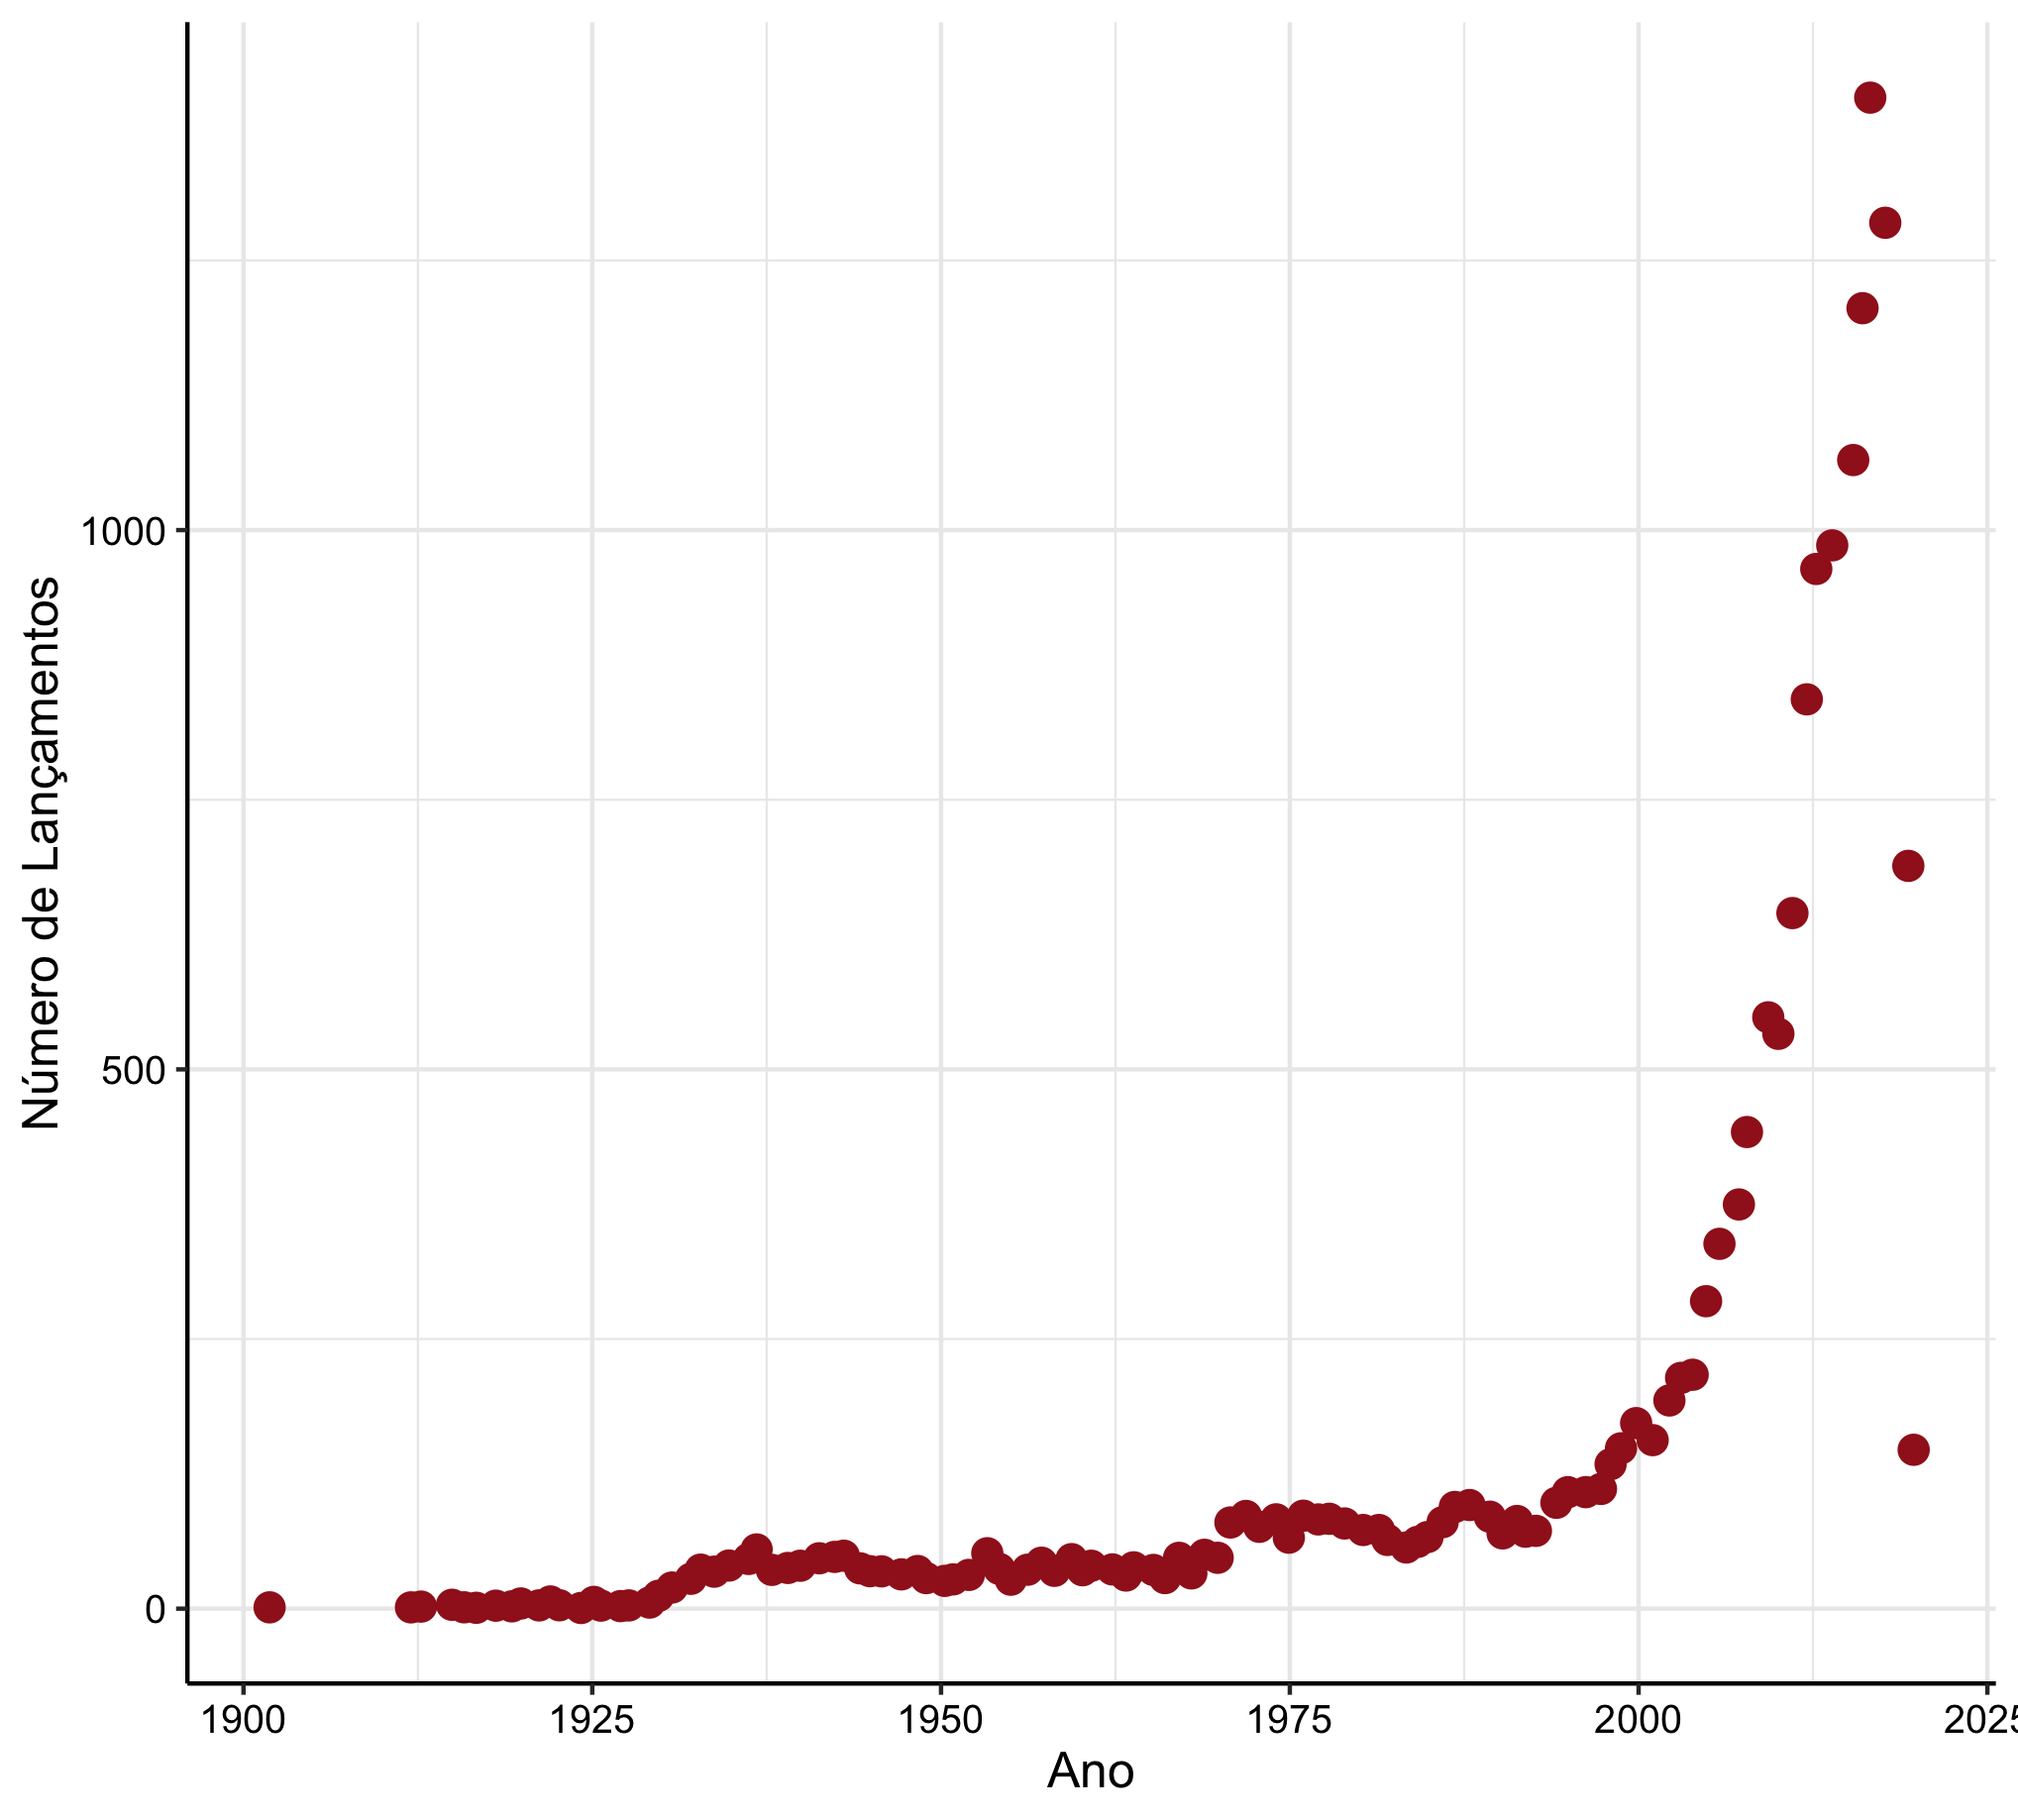
\includegraphics[scale=0.15]{Fig_Lancamentos_Ano.png}
    \label{fig:my_label}
\end{figure}

Na tabela abaixo é possível observar a quantidade de lançamentos por década. 

\begin{table}[H]
\caption{Frequência absoluta da variável Número de Lançamentos ao longo das década}
\centering
\begin{tabular}{l|r}
\hline
\multicolumn{1}{l|}{\textbf{Década}} &
\multicolumn{1}{r}{\textbf{Número de Lançamentos}}\\
\hline
Início do Século & 1\\
Anos 10 & 19\\
Anos 20 & 46\\
Anos 30 & 373\\
Anos 40 & 372\\
Anos 50 & 369\\
Anos 60 & 386\\
Anos 70 & 795\\
Anos 80 & 747\\
Anos 90 & 1104\\
Anos 2000 & 3301\\
Anos 2010 & 9231\\
\hline
\textbf{Total} & {16744}\\
\hline
\end{tabular}
\end{table}

Pode-se observar pelo gráfico e tabelas acima que o número de lançamento cresceu ao longo dos anos e que esse aumento foi mais acelerado a partir dos anos 2000.\\

\subsection{Duração do filme e seu ano de lançamento}

\subsubsection{Tempo como variável contínua}

Essa análise permitiu avaliar se há alguma relação entre o tempo de duração do filme e o ano em que foi lançado. Como havia alguns filmes que apresentavam um tempo de duração muito discrepante em relação aos outros (\emph{outliers}) eles foram removidos dos dados utilizados nessa fase.\\

No gráfico de dispersão abaixo é possível observar essa relação. 

\begin{figure}[H]
    \centering
    \caption{Gráfico de Dispersão duração do filme com o decorrer dos anos}
    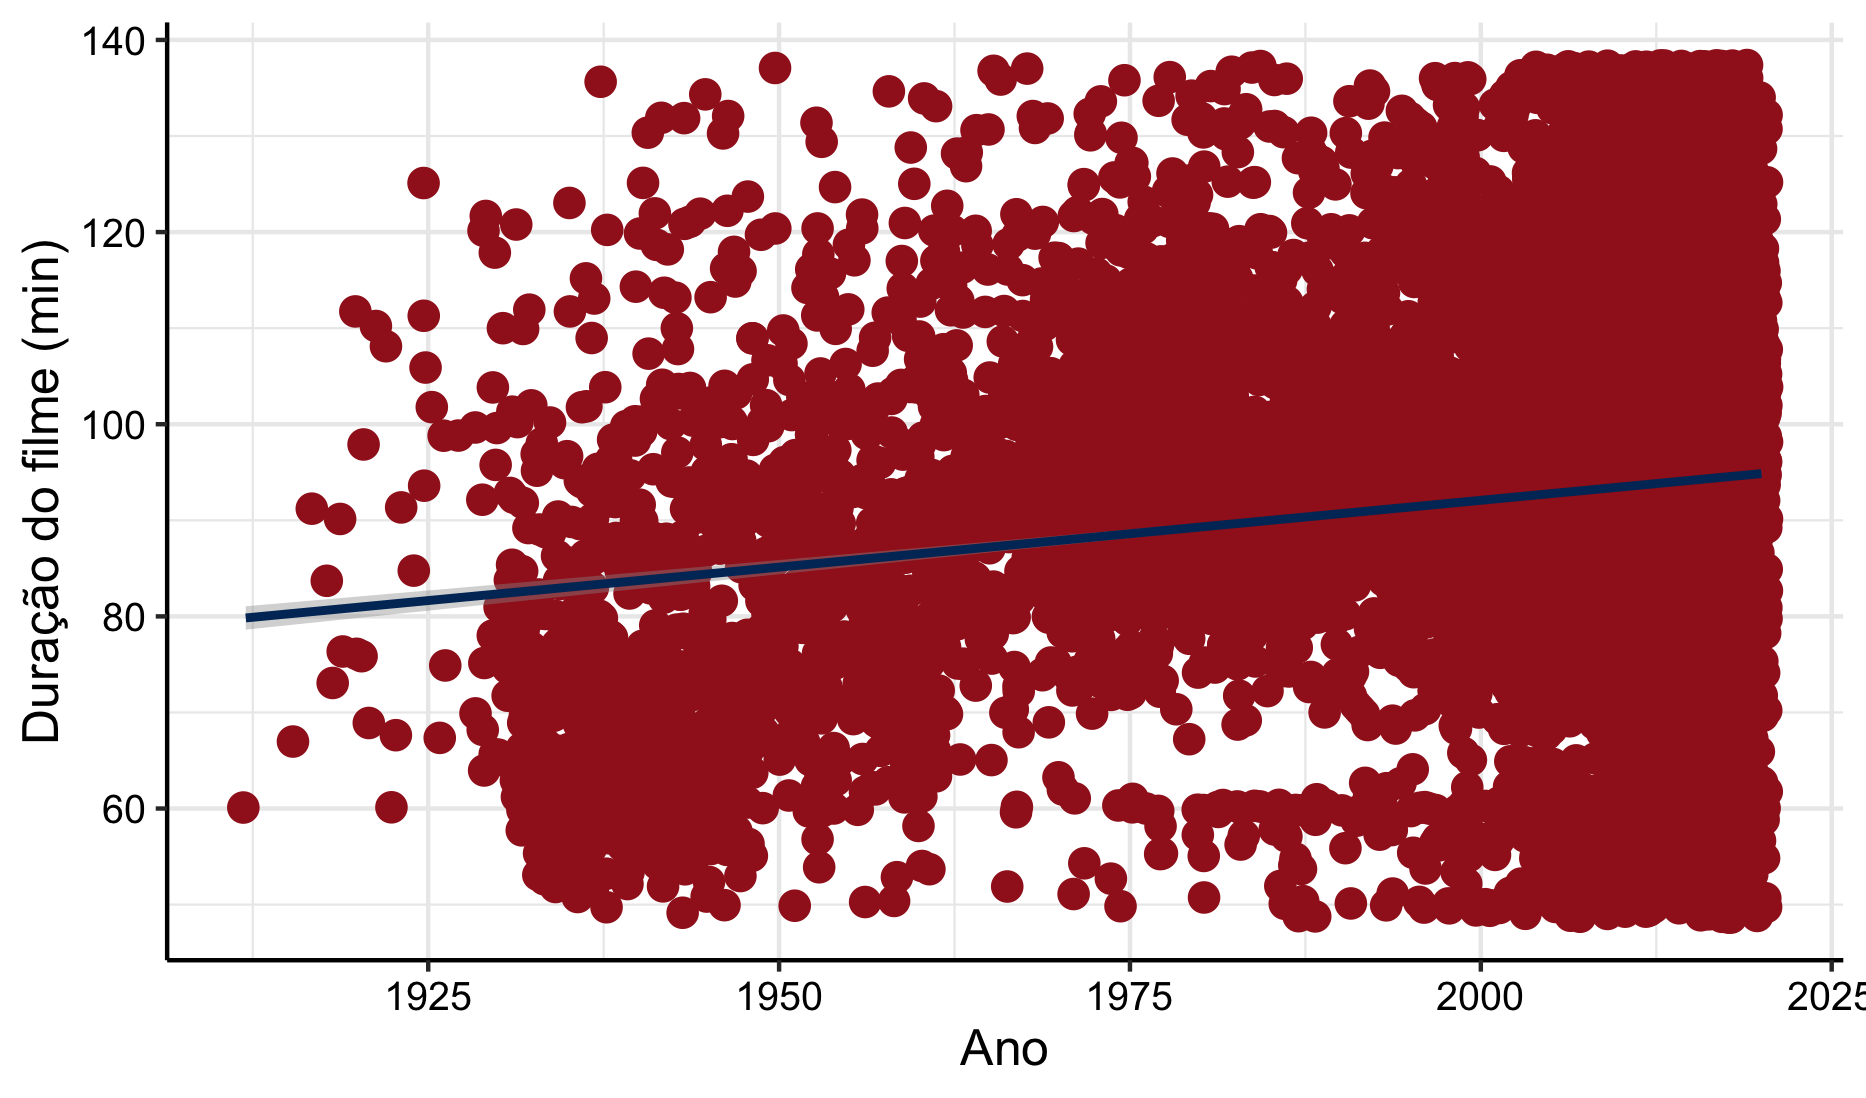
\includegraphics[scale=0.15]{Fig_Duracao_Lancamento.png}
    \label{fig:my_label}
\end{figure}

O gráfico pode parecer um pouco confuso, uma vez que apresenta muita sobreposição de pontos. No entanto, a linha adicionada ao gráfico corresponde à regressão linear para essas variáveis, onde podemos observar uma relação positiva. Os detalhes dessa regressão serão apresentados a seguir. O mesmo padrão pode ser observado na tabela abaixo.

\begin{table}[H]
\caption{Medidas Resumo do tempo de duração (min) dos filmes ao longo das décadas}
\centering
\begin{tabular}{l|rrrrrrrrrr}
\hline
\multicolumn{1}{l|}{\textbf{Década}} &
\multicolumn{1}{r}{\textbf{N}} &
\multicolumn{1}{r}{\textbf{Média}} &
\multicolumn{1}{r}{\textbf{DP}}&
\multicolumn{1}{r}{\textbf{Mínimo}}&
\multicolumn{1}{r}{\textbf{Q1}}&
\multicolumn{1}{r}{\textbf{Mediana}}&
\multicolumn{1}{r}{\textbf{Q3}}&
\multicolumn{1}{r}{\textbf{Máximo}}\\
\hline
Anos 10 & 11  & 82.09 & 14.84 & 60 & 74.5 & 76 & 90.5 & 112\\
Anos 20 & 35  & 89.77 & 19.59 & 60 & 69.5 & 92 & 105.0 & 125\\
Anos 30 & 349  & 72.53 & 15.54 & 50 & 61.0 & 68 & 82.0 & 136\\
Anos 40 & 344  & 78.79 & 18.89 & 49 & 64.0 & 74 & 91.0 & 137\\
Anos 50 & 337  & 84.65 & 16.02 & 50 & 73.0 & 83 & 93.0 & 135\\
Anos 60 & 342 & 93.29 & 14.80 & 52 & 84.0 & 92 & 101.0 & 137\\
Anos 70 & 725  & 94.54 & 13.93 & 50 & 87.0 & 93 & 102.0 & 136\\
Anos 80 & 668  & 94.80 & 14.94 & 49 & 87.5 & 94 & 102.0 & 137\\
Anos 90 & 948  & 94.82 & 15.88 & 49 & 88.0 & 95 & 103.0 & 136\\
Anos 2000 & 2884  & 93.73 & 16.80 & 49 & 85.0 & 93 & 103.0 & 137\\
Anos 2010 & 8039  & 93.12 & 16.96 & 49 & 84.0 & 92 & 103.0 & 137\\
\hline
\end{tabular}
\end{table}

Antes da realização da regressão linear, a normalidade dos dados (sem \emph{outliers}) foi verificada visualmente por meio dos gráficos de densidade, QQplot, a curtose e assimetria, apresentados abaixo. Os parâmetros foram considerados razoavelmente satisfatórios para a realização de uma regressão linear. 

Os gráficos abaixo mostram uma distribuição razoavelmente simétrica (Assimetria de 0.007, indicando uma leve assimetria à direita) e uma distribuição leptocúrtica (Curtose = 3.2, mais fina e comprida em relação à normal). Vemos que a maioria dos filmes tem duração ~90 min, mas que há pequenos picos de filmes com ~60 min e ~120 min.

\begin{figure}[H]
    \centering
    \caption{Gráfico de Dispersão duração do filme com o decorrer dos anos}
    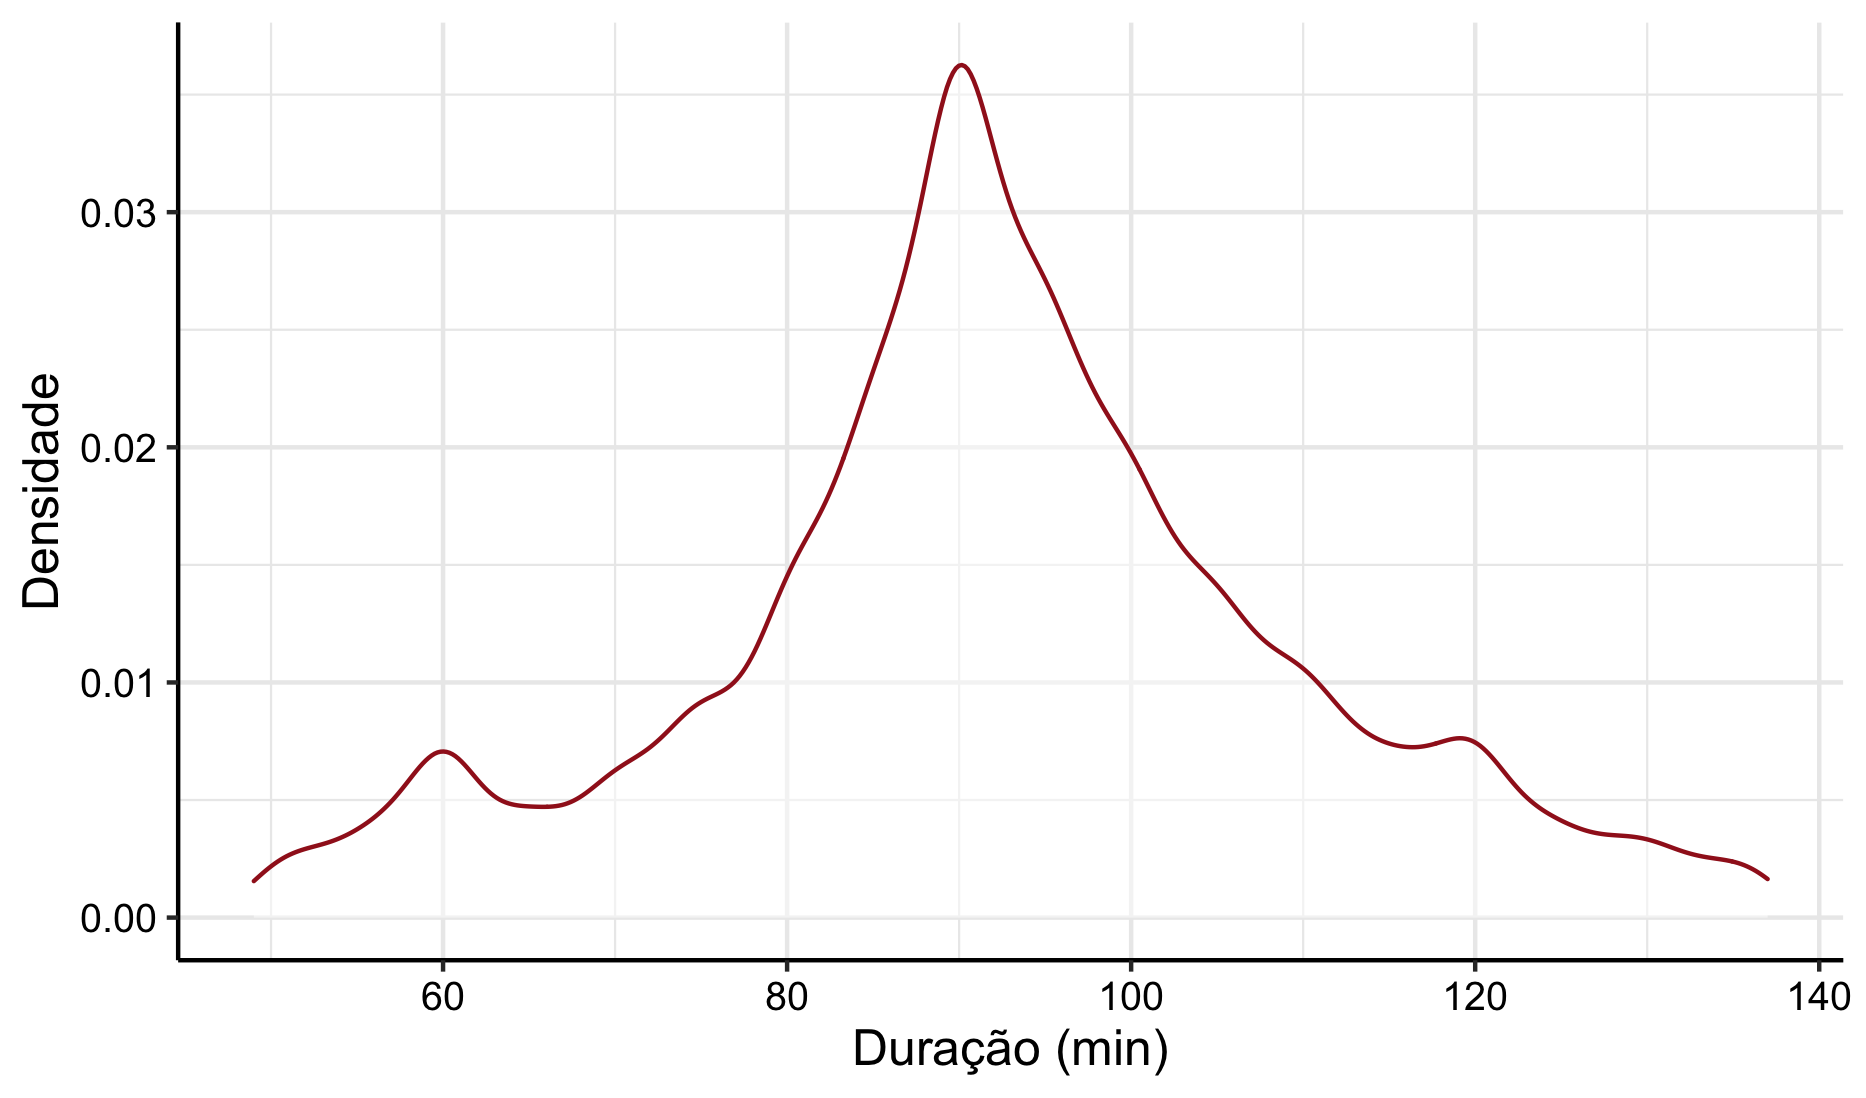
\includegraphics[scale=0.15]{Fig_Duracao_Densidade.png}
    \label{fig:my_label}
\end{figure}

O gráfico abaixo mostra que a distribuição apresenta algum desvio em relação a distribuição normal, entretanto, principalmente para valores intermediários, ela apresenta uma distribuição bem próxima à normalidade. 

\begin{figure}[H]
    \centering
    \caption{Gráfico de Dispersão duração do filme com o decorrer dos anos}
    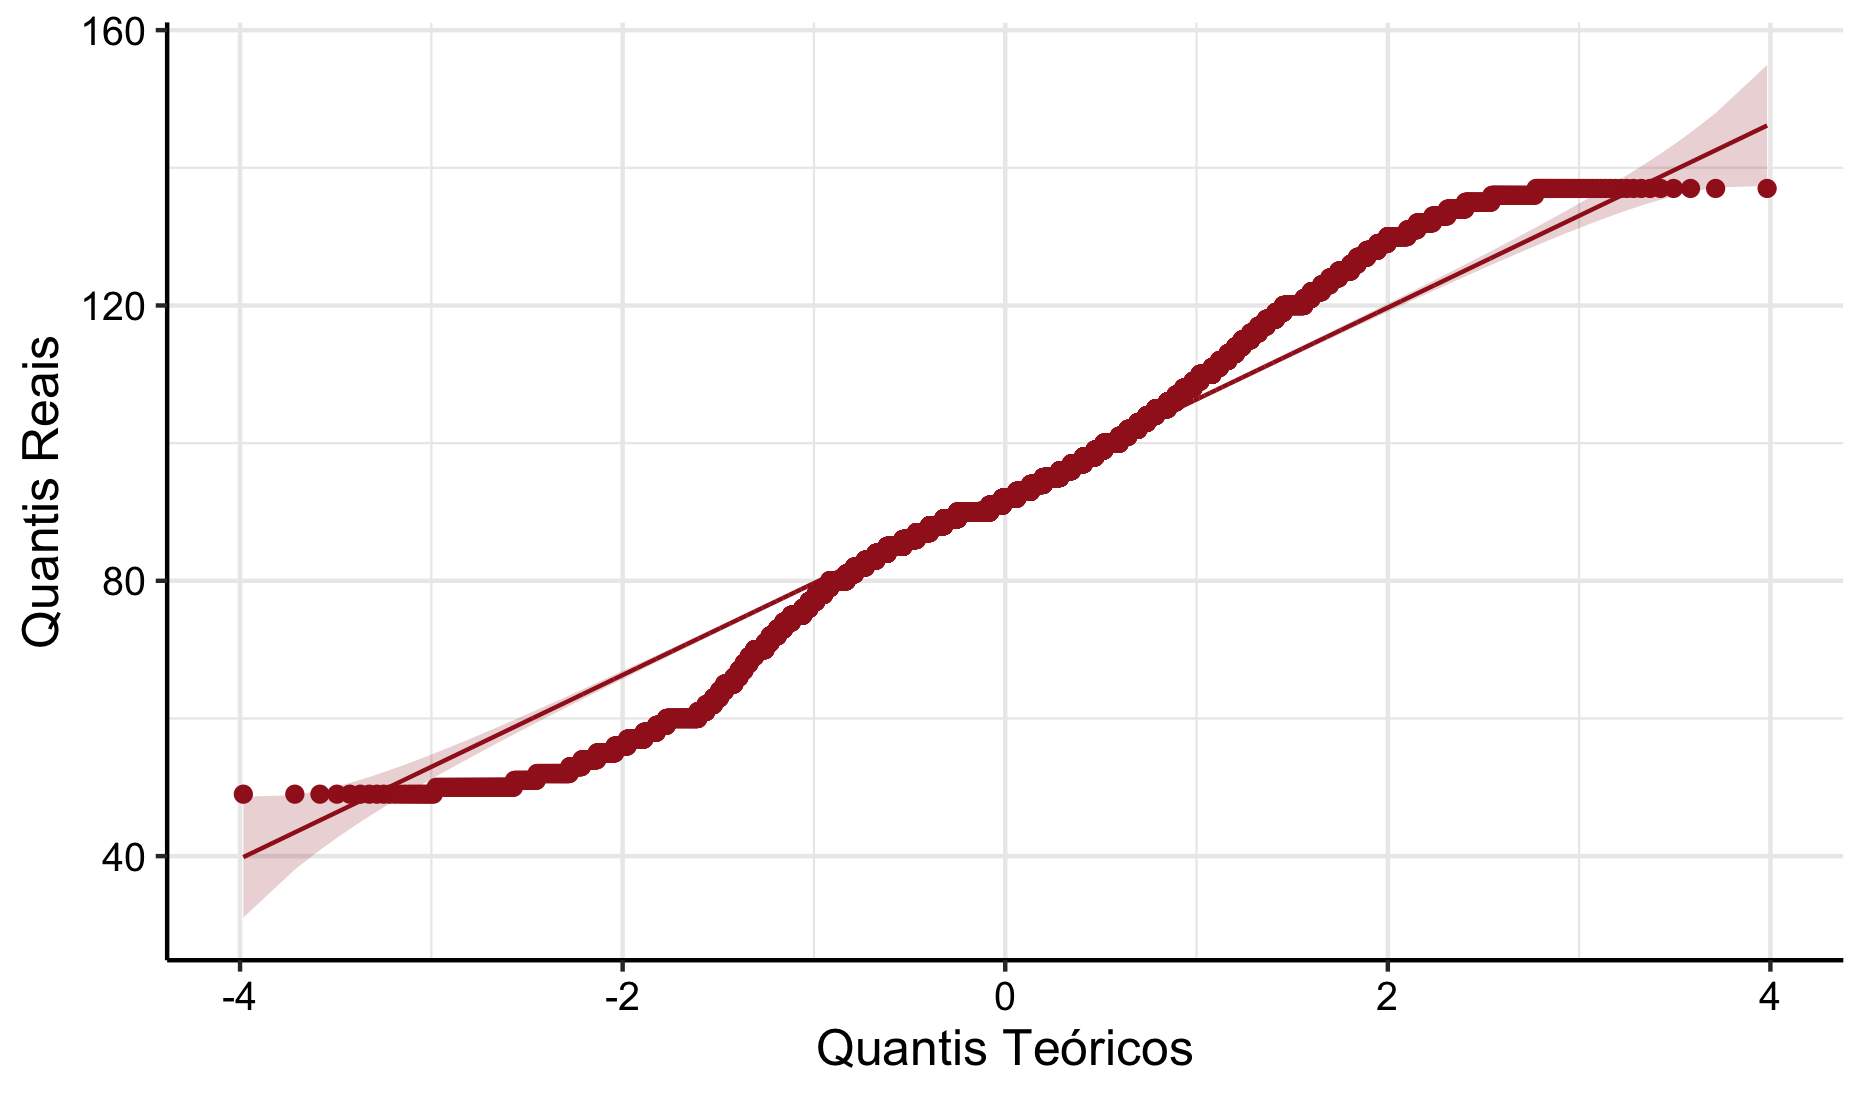
\includegraphics[scale=0.15]{Fig_Duracao_QQ.png}
    \label{fig:my_label}
\end{figure}

Tendo em vista as informações acima, a distribuição foi considerada suficientemente próxima à normal para a realização de uma regressão linear, apesar das diferenças mencionadas. A regressão linear é um método robusto, e esses desvios não foram considerados suficientes para impedir a sua utilização. O resultado do teste de regressão pode ser observado no quadro abaixo:


\begin{quadro}[H]
\centering
\caption{Regressão Linear do tempo de duração em relação ao ano de lançamento}
\label{R-Q-Teste-1}
\vspace{0.1cm}
\resizebox{\textwidth}{!}{
\begin{tabular}{|c|c|c|c|c|}
  \hline
 \textbf{Modelo} & \textbf{Coeficiente}  & \textbf{$R^2$} & \textbf{P-valor} & \textbf{Decisão do Teste} \\ 
  \hline 
  Duração = r*Ano+b & 0.14  & 0.03 & <0.0001 & Rejeita $H_0$\\
  \hline
\end{tabular}}
\end{quadro}

Observando as informações acima, notamos que a variável ano de lançamento e duração do filme tem uma relação positiva significativa. Entretanto, essa relação é fraca, como pode ser observado pelo coeficiente de regressão r e pelo $ R^2$. Ou sejam os filmes aumentaram, em média, em duração ao longo dos anos, mas esse aumento médio não foi acentuado. 

\subsubsection{Tempo como variável categórica}

Para explorar mais afundo essa relação do tempo de duração do filme e o ano de duração, o tempo de duração foi categorizado como descrito na seção de Metodologia. Os gráficos de setores abaixo mostram claramente um aumento na proporção de Longa-Metragem ao longo das décadas. 


\begin{figure}[H]
    \centering
    \caption{Gráfico de Dispersão duração do filme com o decorrer dos anos}
    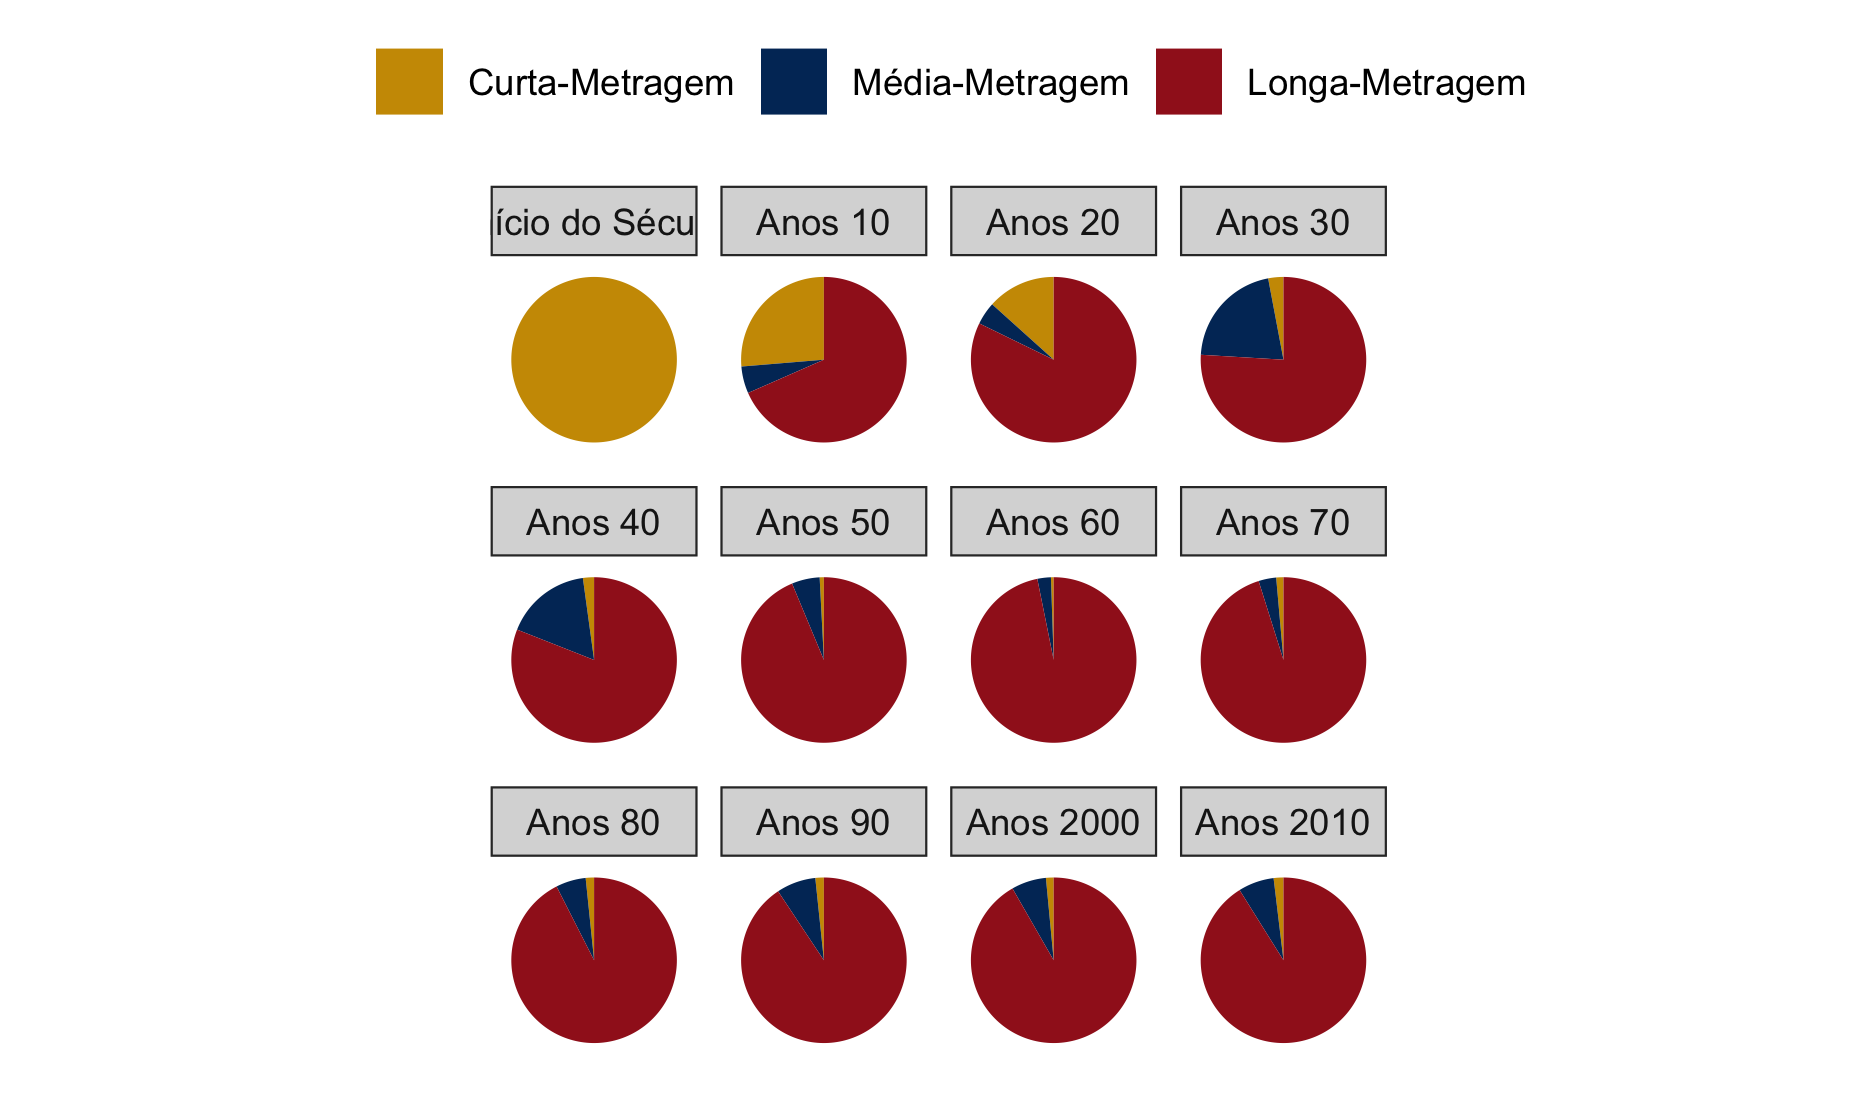
\includegraphics[scale=0.25]{Fig_Setores_Decada_Duracao.png}
    \label{fig:my_label}
\end{figure}

Nas primeiras décadas do século XX (Descontando o primeiro gráfico que indica a produção de um único Curta-Metragem na primeira década), cerca de 25\% das produções se tratavam de Curta-Metragens e 70\% de Longas. Ao início do Século XXI essas proporções eram, respectivamente de 2\% 3 90\%. Essa diferença foi significativa, como está indicado no resultado do teste de $\chi^2$ abaixo:

\begin{quadro}[H]
\centering
\caption{Teste de Associação $\chi^2$ entre as variáveis Metragem e Década }
\label{R-Q-Teste-1}
\vspace{0.1cm}
\resizebox{\textwidth}{!}{
\begin{tabular}{|c|c|c|c|c|}
  \hline
 \textbf{Associação} & \textbf{$\chi^2$}  & \textbf{GL} & \textbf{P-valor} & \textbf{Decisão do Teste} \\ 
  \hline 
  Década x Metragem & 359.16  & 22 & <0.0001 & Rejeita $H_0$\\
  \hline
\end{tabular}}
\end{quadro}

\subsection{Nota do Rotten Tomatoes e o tempo de duração}

\subsubsection{Tempo como variável Contínua}

Neste caso, foi analisado a relação nota  do Rotten Tomatoes para cada tempo de duração. 
 
\begin{figure}[H]
    \centering
    \caption{Gráfico de Dispersão duração do filme com o decorrer dos anos}
    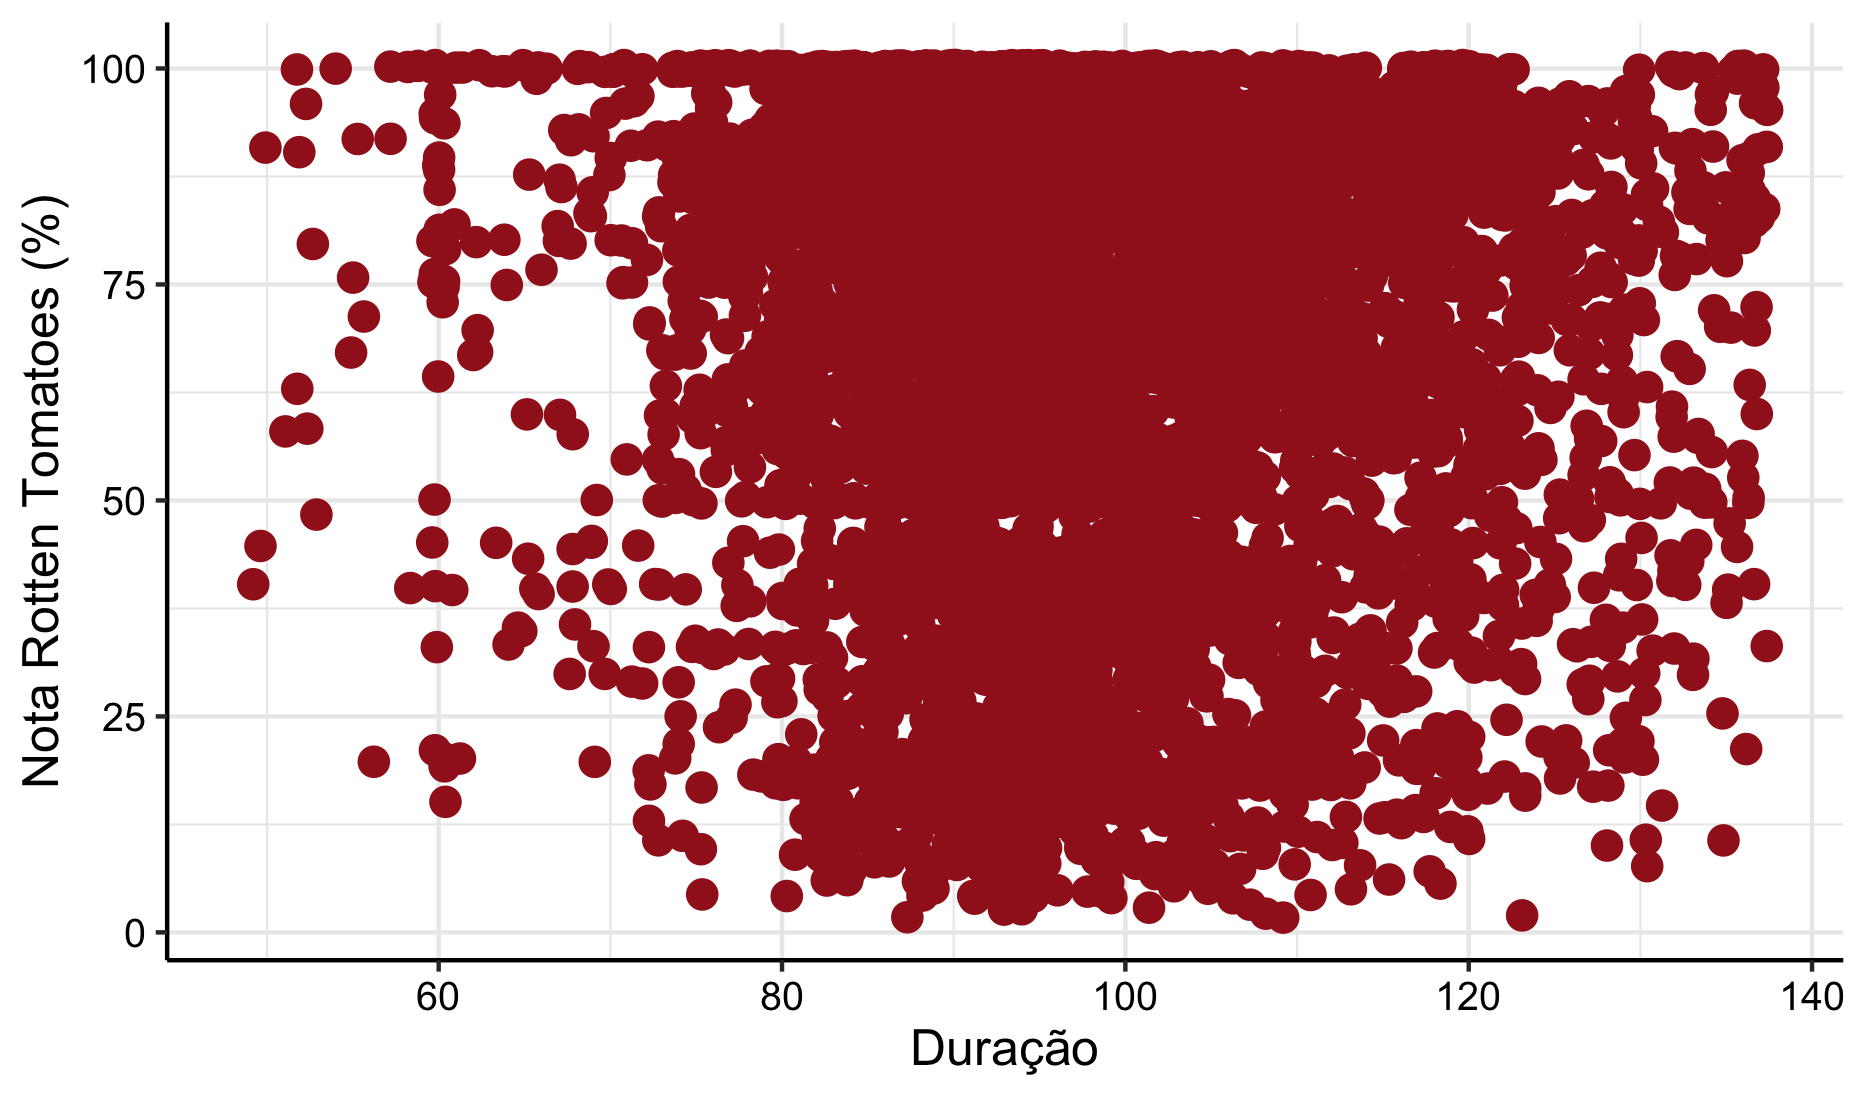
\includegraphics[scale=0.15]{Fig_Rotten_Duracao.png}
    \label{fig:my_label}
\end{figure}

A nota do Rotten Tomatoes não apresenta distribuição normal, como pode ser observada nas figuras e informações abaixo.

\begin{figure}[H]
    \centering
    \caption{Curva de densidade da nota no Rotten Tomatoes }
    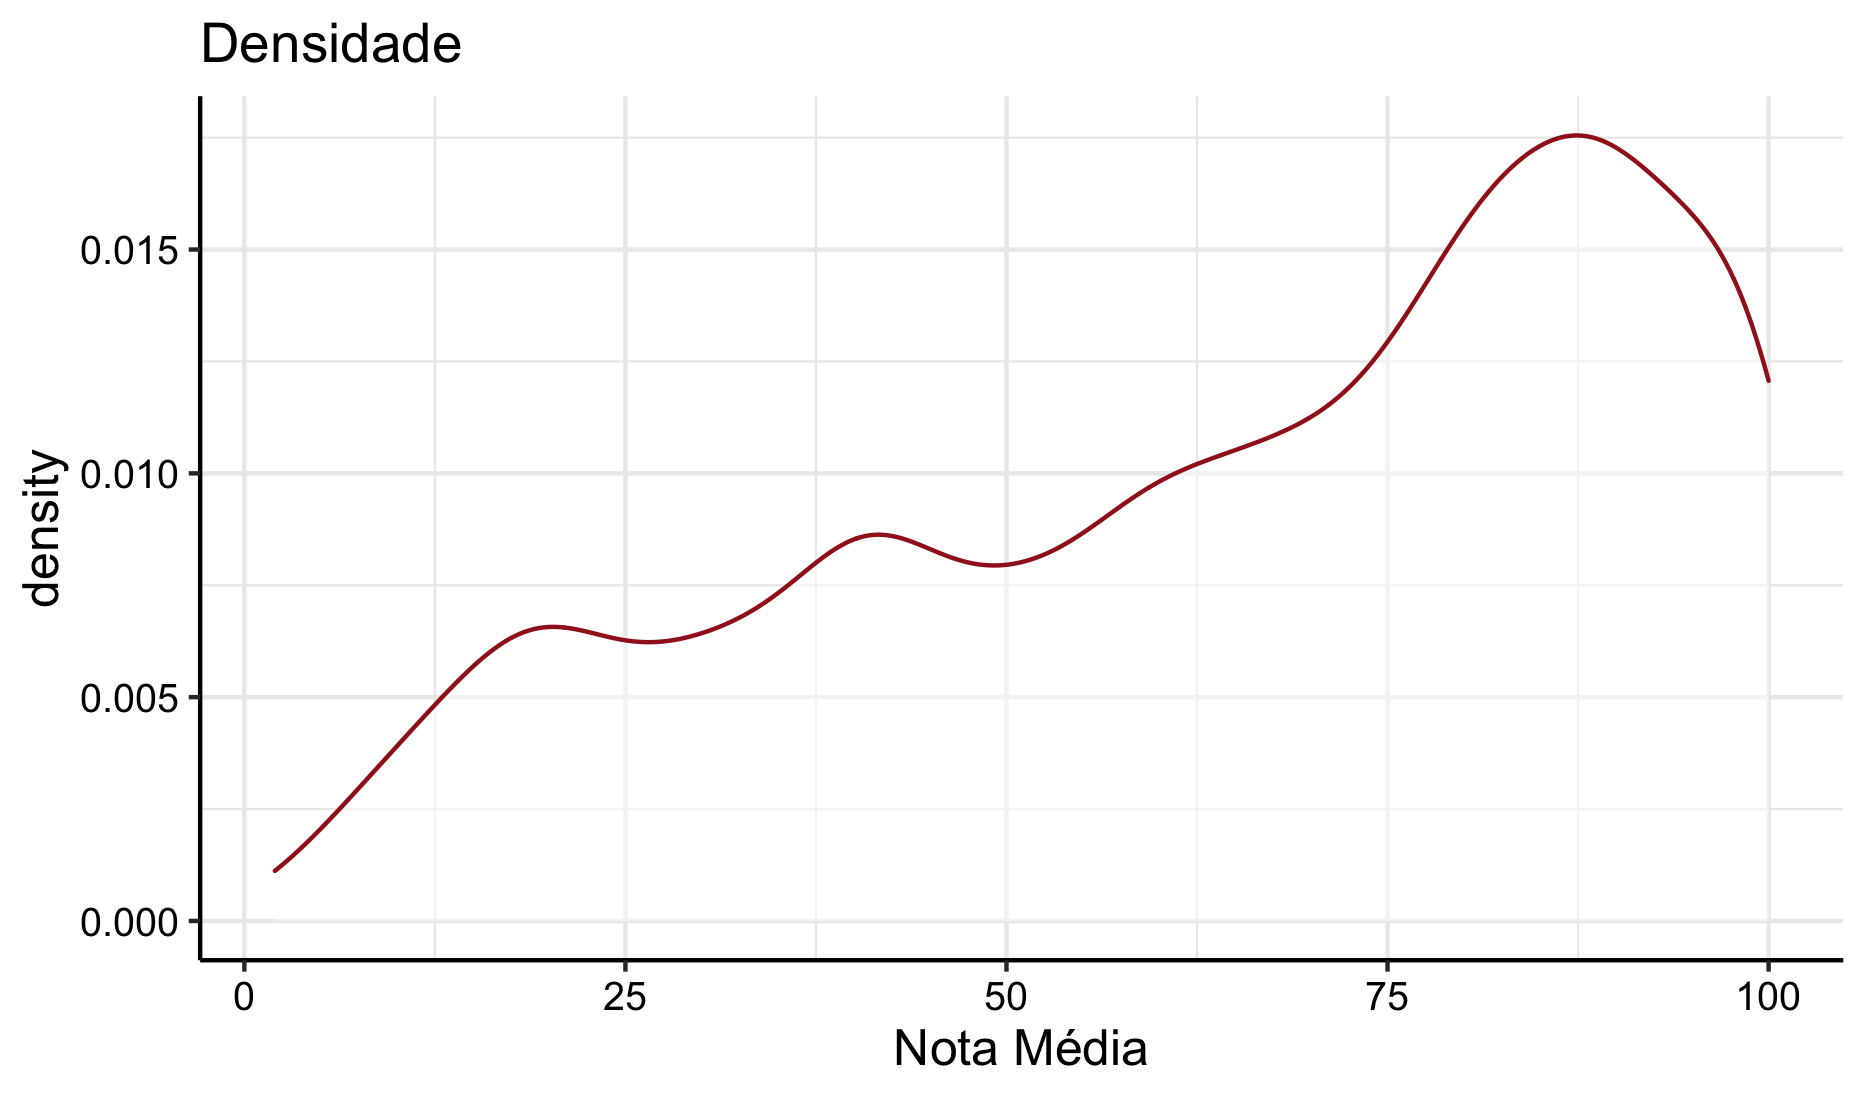
\includegraphics[scale=0.15]{Fig_Rotten_Densidade.png}
    \label{fig:my_label}
\end{figure}

\begin{figure}[H]
    \centering
    \caption{QQ-Plot da nota do Rotten Tomatoes}
    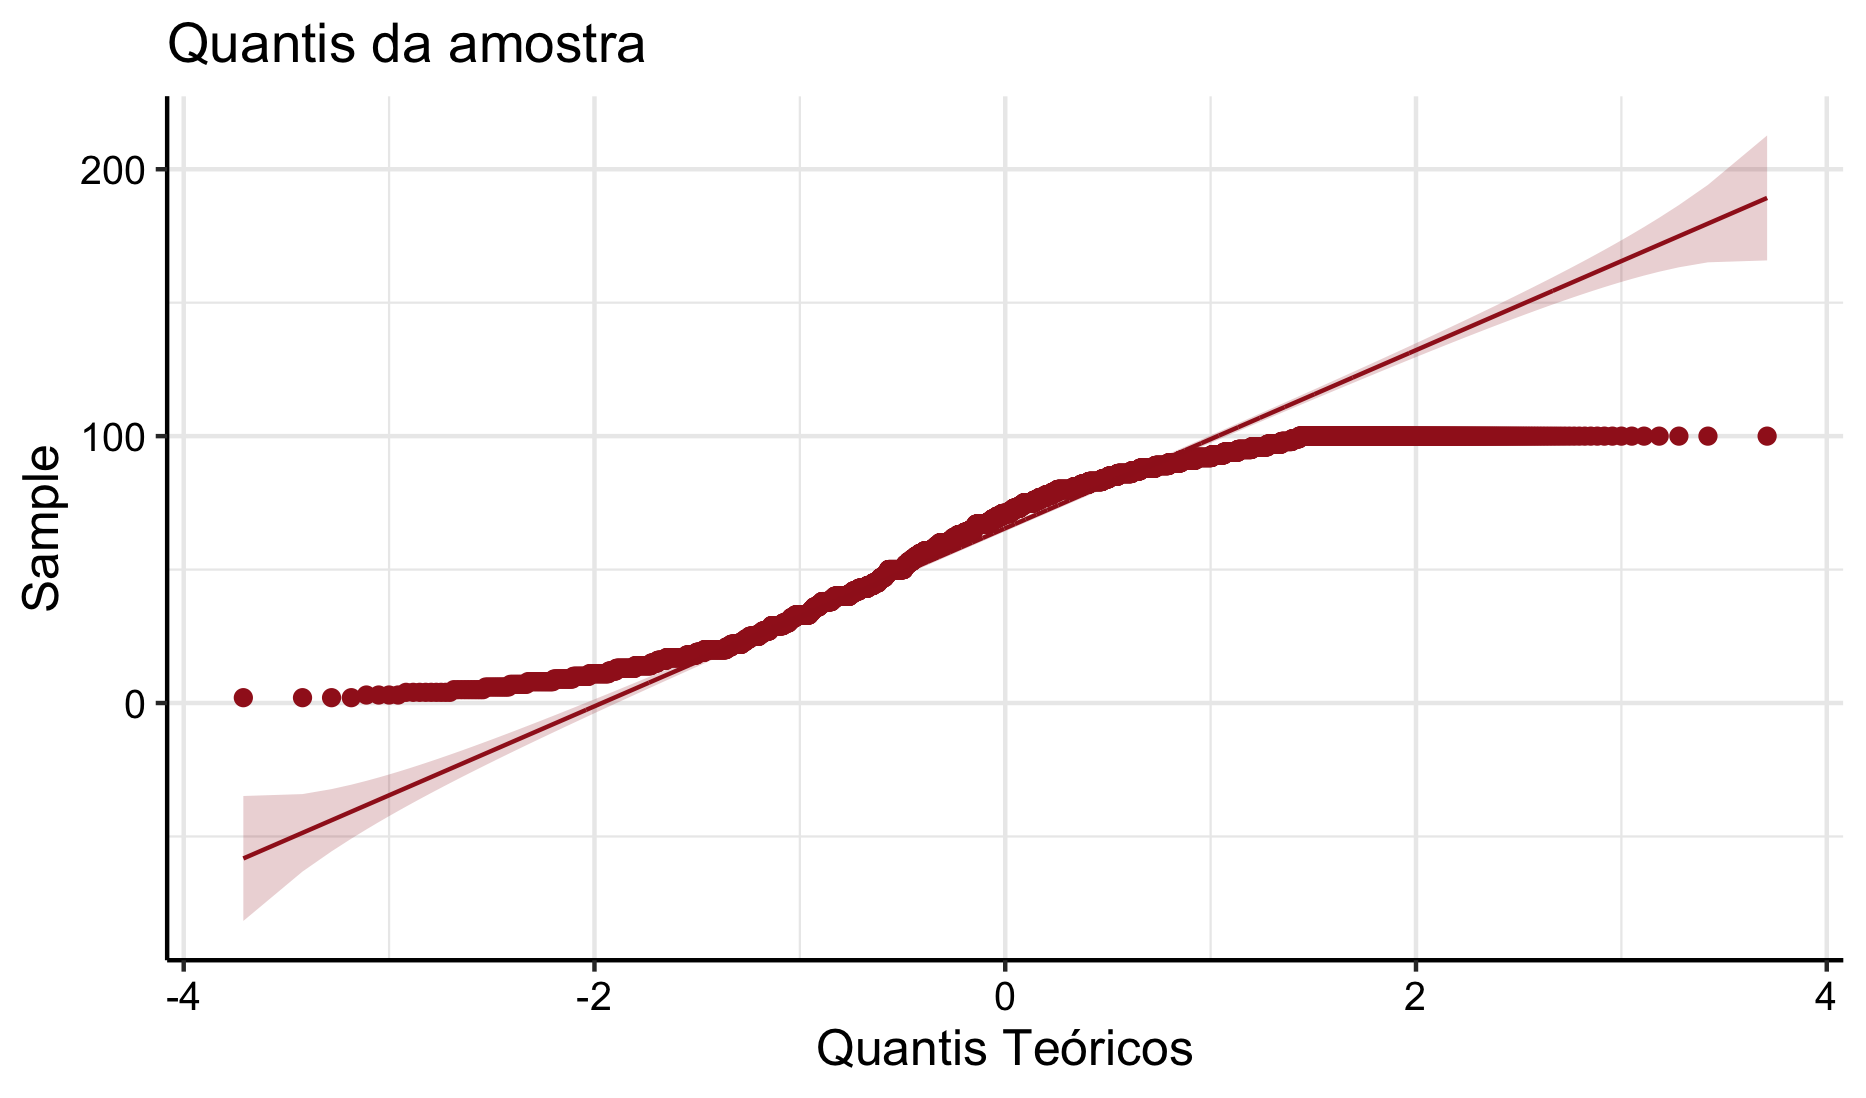
\includegraphics[scale=0.15]{Fig_Rotten_QQ.png}
    \label{fig:my_label}
\end{figure}

Como pode ser observado, a dispersão é notavelmente assimétrica à esquerda (Assimetria -0.5) e Platicúrtica (achatada). Ademais, o QQ-plot mostra um desvio significativo da normal principalmente para os valores em seus extremos. 

Por isso, foi escolhido a o teste Spearman para analisar a correlação entre essas variáveis.
 
\begin{quadro}[H]
\centering
\caption{Teste de Correlação entre as variáveis Tempo de Duração a Avaliação no Rotten Tomatoes }
\label{R-Q-Teste-1}
\vspace{0.1cm}
\resizebox{\textwidth}{!}{
\begin{tabular}{|c|c|c|c|c|}
  \hline
 \textbf{Correlação}  & \textbf{$\rho$} & \textbf{P-valor} & \textbf{Decisão do Teste} \\ 
  \hline 
  Duração x Rotten   & -0.03 & <0.117 & Aceita $H_0$\\
  \hline
\end{tabular}}
\end{quadro}

Como pôde se observado, não uma correlação significativa entre essas variáveis. 

\subsubsection{ Tempo como variável Categórica}

Por outro lado, observando realizando a comparação entre as notas paras os grupos de Curta, Média e Longa-metragens, notamos que os Média-metragens apresentam média de nota no Rotten Tomatoes significativamente maiores.

\begin{figure}[H]
    \centering
    \caption{Boxplot nota do Rotten Tomatoes por Metragem do filme}
    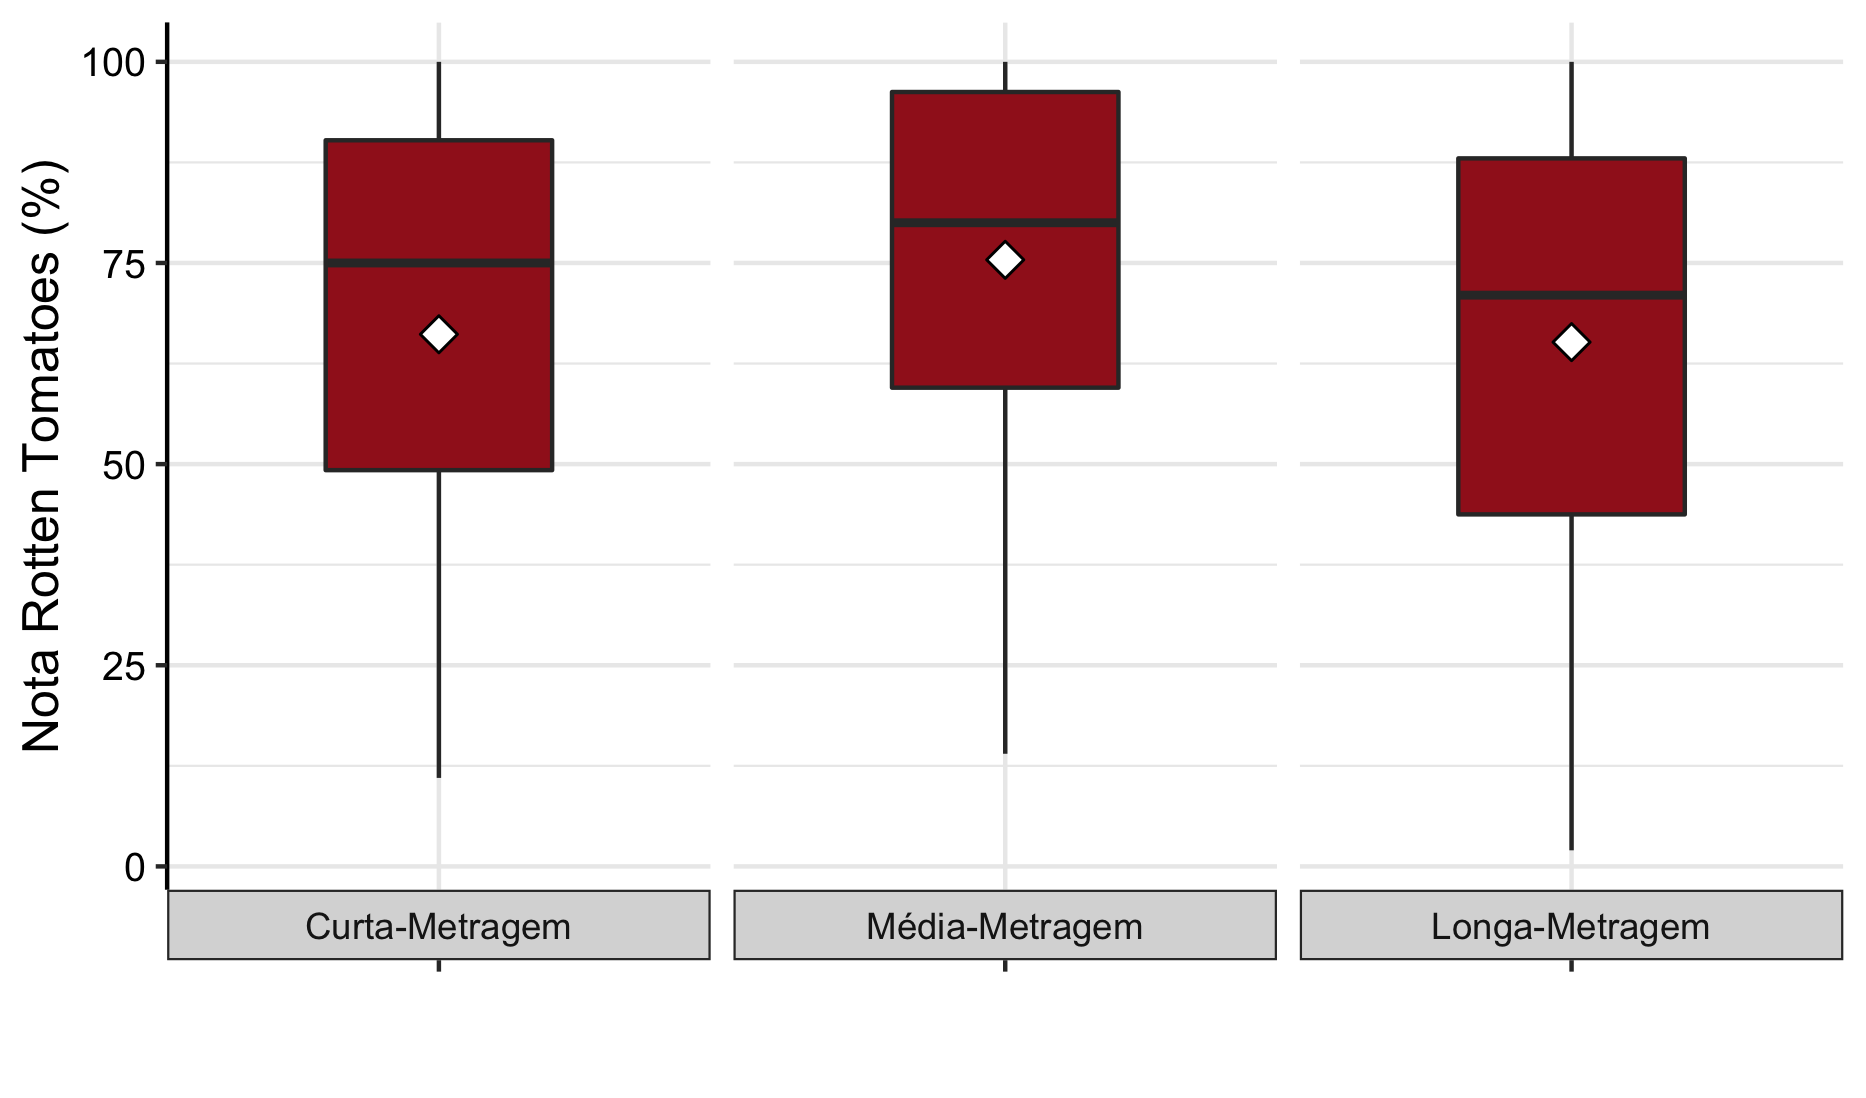
\includegraphics[scale=0.25]{Fig_Rottem_Metragem.png}
    \label{fig:my_label}
\end{figure}

\begin{table}[H]
\caption{Medidas Resumo do tempo de duração dos filmes por categoria de metragem}
\centering
\begin{tabular}{l|rrrrrrrrrr}
\hline
\multicolumn{1}{l|}{\textbf{Metragem}} &
\multicolumn{1}{r}{\textbf{N}} &
\multicolumn{1}{r}{\textbf{Média}} &
\multicolumn{1}{r}{\textbf{DP}}&
\multicolumn{1}{r}{\textbf{Mínimo}}&
\multicolumn{1}{r}{\textbf{Q1}}&
\multicolumn{1}{r}{\textbf{Mediana}}&
\multicolumn{1}{r}{\textbf{Q3}}&
\multicolumn{1}{r}{\textbf{Máximo}}\\
\hline

Curta & 22 & 66.14 & 30.11 &  11 & 49.0 & 75 & 91.0 & 100 \\
Média & 112   & 75.39 & 24.12 &  14 & 59.0 & 80 & 96.5 & 100 \\
Longa &  4988  & 65.16 & 26.65 &  2 & 43.5 & 71 & 88.0 & 100  \\
\hline
\end{tabular}
\end{table}

Uma vez que os dados não apresentam distribuição normal, como mostrado anteriormente, a comparação foi feita pelo teste de Kruskal-Wallis seguido do teste de Dunn.


\begin{quadro}[H]
\centering
\caption{Teste de Kruskal-Wallis comparando as notas do Rotten Tomatoes por tipo de Metragem }
\label{R-Q-Teste-1}
\vspace{0.1cm}
\resizebox{\textwidth}{!}{
\begin{tabular}{|c|c|c|c|c|}
  \hline
 \textbf{Variável}  & \textbf{$\chi^2$} & \textbf{GL}& \textbf{P-valor} & \textbf{Decisão do Teste} \\ 
  \hline 
  Nota Rotten Tomatoes   & 18.675 & 2 & <0.0001 & Rejeita $H_0$\\
  \hline
\end{tabular}}
\end{quadro}

O teste de Dunn mostrou que as notas dos filmes de Média-Metragem são significativamente maiores que os de Longa metragem (p<0.0001).

\subsection{Classificação indicativa do filme por plataforma}

A distribuição de diferentes tipos de classificação indicativa do filme pode ser observada no gráfico abaixo.

\begin{figure}[H]
    \centering
    \caption{Distribuição da Classificação Indicativa por Plataforma}
    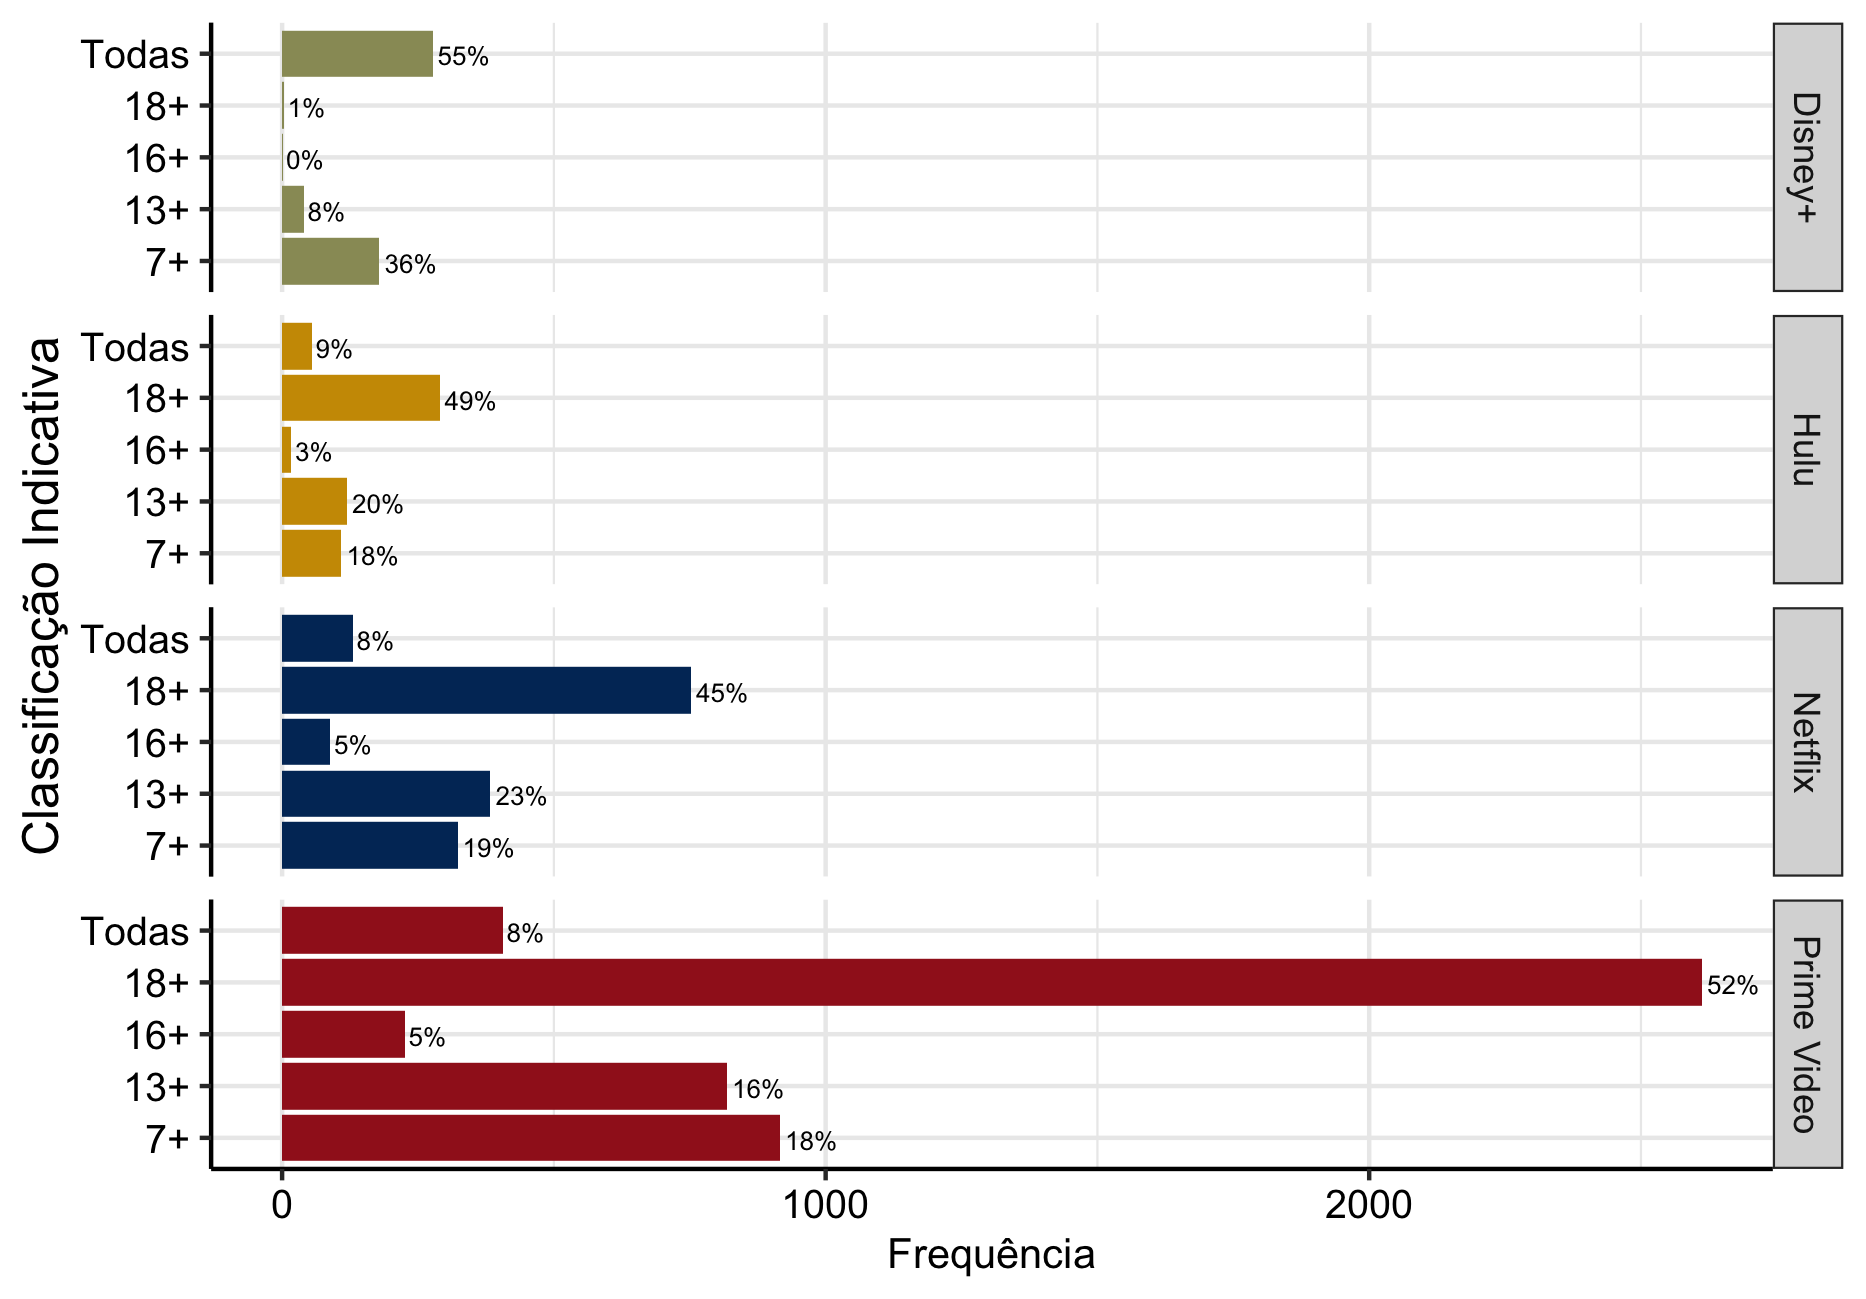
\includegraphics[scale=0.25]{Fig_Classificacao_Plataforma.png}
    \label{fig:my_label}
\end{figure}


\begin{table}[H]
\caption{Medidas Resumo do tempo de duração dos filmes por categoria de metragem}
\centering
\begin{tabular}{l|rrrrrrrr}
\hline
\multicolumn{1}{l|}{\textbf{Classificação}} &
\multicolumn{1}{r}{\textbf{Disney+}} &
\multicolumn{1}{r}{\textbf{\%}} &
\multicolumn{1}{r}{\textbf{Hulu}}&
\multicolumn{1}{r}{\textbf{\%}}&
\multicolumn{1}{r}{\textbf{Netflix}}&
\multicolumn{1}{r}{\textbf{\%}}&
\multicolumn{1}{r}{\textbf{Prime Video}}&
\multicolumn{1}{r}{\textbf{\%}}\\
\hline

 7+ & 179 & 35.8 & 109 & 18.5 & 323 & 19.3 & 916 & 18.4 \\
 13+ &  40 & 8.0 & 119 & 20.2 & 383 & 22.8 & 819 & 16.4 \\
 16+ & 1 & 0.2 & 17 & 2.9 & 89 & 5.3 & 226 & 4.5  \\
 18+ & 3 & 0.6 & 290 & 49.2 & 752 & 44.8 & 2612 & 52.5   \\
Todas &  277 & 55.4 &  55 & 9.3 &  130 & 7.8 &  406 & 8.2  \\
\hline
\end{tabular}
\end{table}

Para a realização de um teste de $\chi^2$ mais fácil de interpretar, a variável Classificação Indicativa foi transformada em uma variável Dicotômica (Menores ou maiores de 18 anos). Observamos uma associação significativa entre a Plataforma e a Classificação, que se diferencia principalmente por uma maior proporção de filmes de Classificação indicativa livre na plataforma Disney+ e em contra partida uma proporção maior de files para maiores de 18 anos na plataforma Prime Video.

\begin{quadro}[H]
\centering
\caption{Teste $\chi^2$ entre classificação e plataforma }
\label{R-Q-Teste-1}
\vspace{0.1cm}
\resizebox{\textwidth}{!}{
\begin{tabular}{|c|c|c|c|c|}
  \hline
 \textbf{Associação}  & \textbf{$\chi^2$} & \textbf{GL}& \textbf{P-valor} & \textbf{Decisão do Teste} \\ 
  \hline 
  Classificação x Plataforma   & 495.59 & 3 & <0.0001 & Rejeita $H_0$\\
  \hline
\end{tabular}}
\end{quadro}


\subsection {Uma comparação nota IMDb entre plataformas}
Uma comparação das notas do IMDb entre as plataformas pode ser observada no gráfico e tabela abaixo:

\begin{figure}[H]
    \centering
    \caption{Nota do IMDb por Plataforma}
    
\includegraphics[scale=0.25]{Fig_IMDb_Plataforma.png}
    \label{fig:my_label}
\end{figure}

\begin{table}[H]
\caption{Medidas Resumo do tempo nota do IMDb por Plataforma}
\centering
\begin{tabular}{l|rrrrrrrrrr}
\hline
\multicolumn{1}{l|}{\textbf{Plataforma}} &
\multicolumn{1}{r}{\textbf{N}} &
\multicolumn{1}{r}{\textbf{Média}} &
\multicolumn{1}{r}{\textbf{DP}}&
\multicolumn{1}{r}{\textbf{Mínimo}}&
\multicolumn{1}{r}{\textbf{Q1}}&
\multicolumn{1}{r}{\textbf{Mediana}}&
\multicolumn{1}{r}{\textbf{Q3}}&
\multicolumn{1}{r}{\textbf{Máximo}}\\
\hline

Disney+ &  500 & 0 &  6.41 & 1.05 &  1.6 & 5.8 & 6.5 & 7.2 & 8.7 \\
Hulu & 585 & 5 &  6.20 & 1.11 & 2.2 & 5.5 & 6.2 & 7.1 & 9.0  \\
Netflix &  1673 & 4 &  6.29 & 1.10 &  2.1 & 5.6 & 6.3 & 7.1 & 8.8  \\
Prime Video &  4950 & 29 & 5.63 & 1.39 & 1.0 & 4.7 & 5.8 & 6.7 & 9.1  \\
\hline
\end{tabular}
\end{table}

Uma vez que o teste de Shapiro-Wilk indicou uma distribuição diferente da normal e o teste de Bartlett indicaram não-homogeneidade das variâncias, foi escolhido um teste de postos de Kruskal-Wallis para comparar os grupos. O teste mostra uma diferença a nota entre as plataformas, sendo que a plataforma Prime Video foi a que apresentou, de nomo geral, as menores notas. Entretanto, é importante ter em mente que essa também foi a plataforma com maior número de filmes em \emph{streaming}, o que amplia as chances de apresentar filmes piores em seu catálogo. O resultado do teste pode ser observado na tabela abaixo:


\begin{quadro}[H]
\centering
\caption{Teste Krukal-Wallis da nota IMDb entre plataforma }
\label{R-Q-Teste-1}
\vspace{0.1cm}
\resizebox{\textwidth}{!}{
\begin{tabular}{|c|c|c|c|c|}
  \hline
 \textbf{Variável}  & \textbf{$\chi^2$} & \textbf{GL}& \textbf{P-valor} & \textbf{Decisão do Teste} \\ 
  \hline 
  Nota IMDb   & 409.2017 & 3 & <0.0001 & Rejeita $H_0$\\
  \hline
\end{tabular}}
\end{quadro}

O teste de Dunn indica que todos grupos são diferentes entre si, exceto Hulu x Netflix.

\subsection {Top 5 diretores de acordo com a nota IMDb}

Esta questão pode ser avaliada de diversas formas:

\subsubsection{Quais eram os diretores dos filmes com as cinco maiores notas no IMDb?}

A Classificação para um filme individual se deu como se segue:\\

\begin{enumerate}[topsep=0pt,partopsep=0pt]
\item Fen Tian, com nota 9.3 pelo filme \emph{ Love on a Leash}
\item Danny Wu , com nota 9.3  pelo filme \emph{Square One}  
\itemTom McLoughlin, com nota  9.3 pelo filme \emph{Steven Banks: Home Entertainment Center}
\item Miguel Gaudêncio, com nota  9.3 pelo filme \emph{Down, But Not Out!}            
\item Roger Donaldson, com nota  9.3 pelo filme \emph{Bounty}      
\end{enumerate}

\subsubsection{Qual as cinco melhores notas médias dos diretores?}

Para essa análise foram considerados apenas os diretores com pelo menos três filmes:

\begin{enumerate}[topsep=0pt,partopsep=0pt]
    \item Rocco Urbisci
    \item Nick Nanton
    \item Bruce Gowers
    \item Christopher Nolan
    \item Kerry Shawcross
\end{enumerate}



\subsubsection{Qual as cinco melhores notas médias dos filmes com apenas um diretor?}

Na base de dados estudada, há filmes com até mais de 20 diretores. Avaliar aqueles filmes que tiveram apenas um diretor pode ser mais informativo a respeito mo mérito individual. Nesse caso a lista dos Top 5 é composta por:\\

\begin{enumerate}[topsep=0pt,partopsep=0pt]
    \item Rocco Urbisci
    \item Christopher Nolan
    \item Louis C.K.
    \item Rajkumar Hirani
    \item Steven J. Santos
\end{enumerate}

\subsubsection{Qual as cinco melhores notas médias dos filmes com apenas um diretor, para cada gênero de filmes?}

Finalmente, é interessante analisar esse ranking para gêneros distintos de filmes. Alguns exemplos podem ser observados abaixo:\\

\textbf{Drama}
\newline

\begin{enumerate}[topsep=0pt,partopsep=0pt]
    \item Mani Ratnam
    \item Martin Scorsese
    \item Rajkumar Hirani
    \item Hrishikesh Mukherjee
    \item David Batty
\end{enumerate}\\

\pagebreak

\textbf{Ação e Aventura}
\newline

\begin{enumerate}[topsep=0pt,partopsep=0pt]
    \item Christopher Nolan
    \item Quentin Tarantino
    \item S.S. Rajamoul
    \item Toshiyuki Kubooka
    \item Werner Herzog
\end{enumerate}\\

\textbf{Comédia}
\newline

\begin{enumerate}[topsep=0pt,partopsep=0pt]
    \item Rocco Urbisci
    \item Hrishikesh Mukherjee
    \item Louis C. K.
    \item Steven J. Santos.
    \item Stan Lathan
\end{enumerate}\\
\textbf{Ficção Científica e Fantasia}
\newline

\begin{enumerate}[topsep=0pt,partopsep=0pt]
    \item Toshiyuki Kubooka
    \item Gore Verbinski
    \item Robert Zemeckis
    \item George Lucas
    \item Steven Spielberg
\end{enumerate}\\

Levando em consideração todos os gêneros presentes no banco, os diretores que mais frequentemente apareceram na lista dos Top 5 pela nota do IMDb podem ser visualizados na nuvem de palavras abaixo:\\

\begin{figure}[H]
    \centering
    \caption{Nuvem de Palavras por Diretor em Diferentes Gêneros}
    
\includegraphics[scale=1]{Nuvem.png}
    \label{fig:my_label}
\end{figure}

\pagebreak

\section{Conclusões}
\textbf{Ficção Científica e Fantasia}
\begin{enumerate}[topsep=0pt,partopsep=0pt]
    \item Os lançamentos de filmes aumentaram com o passar dos anos, principalmente após os anos 2000.
    \item A duração do filme está fracamente, mas significativamente, relacionada de forma positiva com os anos. Ou seja, filmes mais recentes tendem a ser de maior duração. Também teve um aumento na proporção de Longa-metragens em anos mais recentes. 
    \item Não houve associação direta entre o tempo de duração do filme e a nota no Rotten Tomatoes, mas os Média-Metragens apresentaram notas significativamente maiores. 
    \item A plataforma Disney+ foi a que apresentou maior proporção de filmes de classificação livre, enquanto a Prime Video apresentou maior proporção de filmes para maiores de 18 anos. 
    \item A plataforma Prime Video foi a que apresentou menor pontuação média de seus filmes no IMDb, enquanto a Disney+ apresentou a maior. 
    \item Entre os diretores mais frequentemente presentes nos Top5, e mais conhecidos no ocidente, estão Quentin Tarantino, Christopher Nolan e Martin Scorsese.
\end{enumerate}


\end{document}